\documentclass[11pt,a4paper]{article}
\usepackage[spanish,es-nodecimaldot]{babel}	% Utilizar español
\usepackage[utf8]{inputenc}					% Caracteres UTF-8
\usepackage{graphicx}						% Imagenes
\usepackage[hidelinks]{hyperref}			% Poner enlaces sin marcarlos en rojo
\usepackage{fancyhdr}						% Modificar encabezados y pies de pagina
\usepackage{float}							% Insertar figuras
\usepackage[textwidth=390pt]{geometry}		% Anchura de la pagina
\usepackage[nottoc]{tocbibind}				% Referencias (no incluir num pagina indice en Indice)
\usepackage{enumitem}						% Permitir enumerate con distintos simbolos
\usepackage[T1]{fontenc}					% Usar textsc en sections
\usepackage{amsmath}						% Símbolos matemáticos
\usepackage{natbib}
\usepackage{subcaption}

% Comando para poner el nombre de la asignatura
\newcommand{\asignatura}{Visión por Computador}
\newcommand{\autor}{Vladislav Nikolov Vasilev}
\newcommand{\titulo}{Práctica 2}
\newcommand{\subtitulo}{Redes Neuronales Convolucionales}

\usepackage{listings}
\usepackage{xcolor}
 
\definecolor{codegreen}{rgb}{0,0.6,0}
\definecolor{codegray}{rgb}{0.5,0.5,0.5}
\definecolor{codepurple}{rgb}{0.58,0,0.82}
\definecolor{backcolour}{rgb}{0.95,0.95,0.92}
 
\lstdefinestyle{mystyle}{
    backgroundcolor=\color{backcolour},   
    commentstyle=\color{codegreen},
    keywordstyle=\color{magenta},
    numberstyle=\tiny\color{codegray},
    stringstyle=\color{codepurple},
    basicstyle=\ttfamily\footnotesize,
    breakatwhitespace=false,         
    breaklines=true,                 
    captionpos=b,                    
    keepspaces=true,                 
    numbers=left,                    
    numbersep=5pt,                  
    showspaces=false,                
    showstringspaces=false,
    showtabs=false,                  
    tabsize=4,
    language=Python,
    literate={ñ}{{\~n}}1
}

\lstset{style=mystyle}

% Configuracion de encabezados y pies de pagina
\pagestyle{fancy}
\lhead{\autor{}}
\rhead{\asignatura{}}
\lfoot{Grado en Ingeniería Informática}
\cfoot{}
\rfoot{\thepage}
\renewcommand{\headrulewidth}{0.4pt}		% Linea cabeza de pagina
\renewcommand{\footrulewidth}{0.4pt}		% Linea pie de pagina


\begin{document}
\pagenumbering{gobble}

% Pagina de titulo
\begin{titlepage}

\begin{minipage}{\textwidth}

\centering

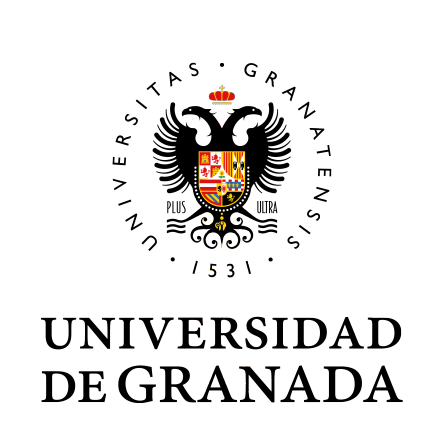
\includegraphics[scale=0.5]{img/ugr.png}\\

\textsc{\Large \asignatura{}\\[0.2cm]}
\textsc{GRADO EN INGENIERÍA INFORMÁTICA}\\[1cm]

\noindent\rule[-1ex]{\textwidth}{1pt}\\[1.5ex]
\textsc{{\Huge \titulo\\[0.5ex]}}
\textsc{{\Large \subtitulo\\}}
\noindent\rule[-1ex]{\textwidth}{2pt}\\[3.5ex]

\end{minipage}

\vspace{0.5cm}

\begin{minipage}{\textwidth}

\centering

\textbf{Autor}\\ {\autor{}}\\[2.5ex]
\textbf{Rama}\\ {Computación y Sistemas Inteligentes}\\[2.5ex]
\vspace{0.3cm}


\includegraphics[scale=0.3]{img/etsiit.jpeg}

\vspace{0.7cm}
\textsc{Escuela Técnica Superior de Ingenierías Informática y de Telecomunicación}\\
\vspace{1cm}
\textsc{Curso 2019-2020}
\end{minipage}
\end{titlepage}

\pagenumbering{arabic}
\tableofcontents
\thispagestyle{empty}				% No usar estilo en la pagina de indice

\newpage

\setlength{\parskip}{1em}

\section{\textsc{BaseNet en CIFAR100}}

Antes de empezar con la traducción de la arquitectura proporcionada de \textit{BaseNet}, hace falta establecer la forma
de la entrada de la primera capa de la red. Esto es necesario, ya que el modelo necesita conocer dicho tamaño para poder
ser compilado sin ningún tipo de error. Como las imágenes de \textit{CIFAR100} tienen un tamaño de $32 \times 32$
píxels, y tienen 3 canales, la dimensión de la entrada va a ser la siguiente:

\begin{lstlisting}
# Tamaño de la entrada
input_shape = (32, 32, 3)
\end{lstlisting}

Una vez definida la forma de la entrada, ya se puede empezar a hacer la traducción a código. El resultado es el siguiente:

\begin{lstlisting}
# Creacion del modelo
model = Sequential()
model.add(Conv2D(6, kernel_size=(5, 5), padding='valid',
				 input_shape=input_shape))
model.add(Activation('relu'))
model.add(MaxPooling2D(pool_size=(2, 2)))

model.add(Conv2D(16, kernel_size=(5, 5), padding='valid'))
model.add(Activation('relu'))
model.add(MaxPooling2D(pool_size=(2, 2)))

model.add(Flatten())
model.add(Dense(units=50))
model.add(Activation('relu'))
model.add(Dense(units=25))
model.add(Activation('softmax'))
\end{lstlisting}

BaseNet es un modelo secuencial, así que empezamos indicando eso. A continuación, añadimos el primer módulo convolucional.
Este se compone de una convolución 2D con un \textit{kernel} de $5 \times 5$, una función de activación no lineal (RELU en
este caso) y un MaxPooling de tamaño $2 \times 2$. El parámetro $padding = valid$ de $Conv2D$ indica que solo se tiene que
aplicar la convolución allá donde se pueda ajustar el \textit{kernel}; es decir, como en las regiones de los bordes no se
puede, se van a ignorar estas zonas, lo cuál implica que la salida no va a tener el mismo tamaño que la entrada. Este módulo
convolucional se repite otra vez. Después de eso, nos encontramos con las capas densas, las cuáles van a actuar como
clasificador. La capa $Flatten$ es necesario ponerla, ya que coge la salida de la anterior, la cuál es un bloque de tamaño
$5 \times 5 \times 16$ (16 imágenes $5 \times 5$), y aplana dicho bloque, convirtiéndolo en un vector de 400 características,
el cuál sirve como entrada al modelo denso. La última capa, la de activación \textit{softmax} es la que va a dar la salida,
un vector de probabilidades para cada clase. En este caso, la salida va a ser un vector de 25 posiciones, ya que estamos
en un problema donde hay 25 clases.

Con el modelo ya definido, y antes de compilarlo, tenemos que establecer algunas cosas más:

\begin{itemize}
	\item \textbf{Optimizador}. El optimizador que se va a utilizar en este caso es el \textbf{SGD} o \textit{Stochastic
	Gradient Descent}. 	Este es uno de los optimizadores más populares e importantes dentro del \textit{machine learning}.
	Se utiliza mucho con redes neuronales, ya sean redes normales o profundas, y es conocido por su robustez y por ofrecer
	unos muy buenos resultados	en general, además de ser bastante rápido a diferencia de otros optimizadores, como por ejemplo
	Adam. En este caso, se va a utilizar con los parámetros por defecto. Es decir, se tendrá un \textit{learning rate} de 0.01,
	y no se utilizará momentum ni el momentum de Nesterov. Estos parámetros parecen razonables, ya que el \textit{learning
	rate} no es ni demasaido pequeño ni demasiado grande. Además, como es un poco difícil ajustar el momento, se ha preferido
	no tocar este parámetro.
	\item \textbf{Tamaño del \textit{batch}}. Otro elemento muy importante a determinar es el tamaño del \textit{batch}, si bien
	no es necesario conocerlo en el momento en el que se compila el modelo. Para un problema como este, teniendo en cuenta que
	tenemos unos 11250 datos de entrenamiento, un tamaño de \textit{batch} razonable es de 32. Este es un tamaño muy utilizado,
	ya que en general ofrece unos buenos resultados, ya que permite converger a buenos óptimos y hace que el modelo
	generalice bastante bien. Con un tamaño menor se estaría explorando demasiado el espacio, mientras que con uno mayor se
	estaría explotando una zona del espacio, lo cuál puede llegar a producir problemas, como que no se generalice demasiado
	bien \cite{DBLP:journals/corr/KeskarMNST16}, cosa que no nos interesa.
	\item \textbf{Número de épocas}. Éste es quizás el parámetro más difícil de decidir a priori, ya que no tenemos mucha
	información. Por tanto, ya que a medida que vayamos haciendo pruebas podremos ver las curvas de entrenamiento y validación,
	podremos decidir en función de éstas cuántas épocas debemos entrenar los modelos. Para empezar, podemos fijar unas 30 épocas,
	ya que parece un número razonable.
\end{itemize}

Con esto ya visto, podemos compilar nuestro modelo. Lo primero que tenemos que hacer es definir el optimizador. Como vamos
a utilizar SGD, lo hacemos de la siguiente forma:

\begin{lstlisting}
# Establecer optimizador a utilizar
optimizer = SGD()
\end{lstlisting}

Para compilar el modelo, lo haremos de la siguiente forma:

\begin{lstlisting}
# Compilar el modelo
model.compile(
    loss=keras.losses.categorical_crossentropy,
    optimizer=optimizer,
    metrics=['accuracy']
)
\end{lstlisting}

Como estamos en un problema de clasificación y la salida que va a dar el modelo es un vector de probabilidades para múltiples
clases, especificamos que la función de pérdida que se utilizará es la entropía cruzada o \textit{Categorical Cross-Entropy},
la cuál es muy utilizada en problemas de clasificación para múltples clases. Especificamos también cuál será el optimizador
a utilizar, e indicamos que la métrica que nos interesa es la precisión o \textit{accuracy}, que representa la proporción
de aciertos sobre el número total de elementos. Existen muchas otras métricas que se pueden utilizar, pero la \textit{accuracy}
es la más sencilla de entender.

Con el modelo ya compilado, podemos visualizarlo de la siguiente forma:

\begin{figure}[H]
  \centering
  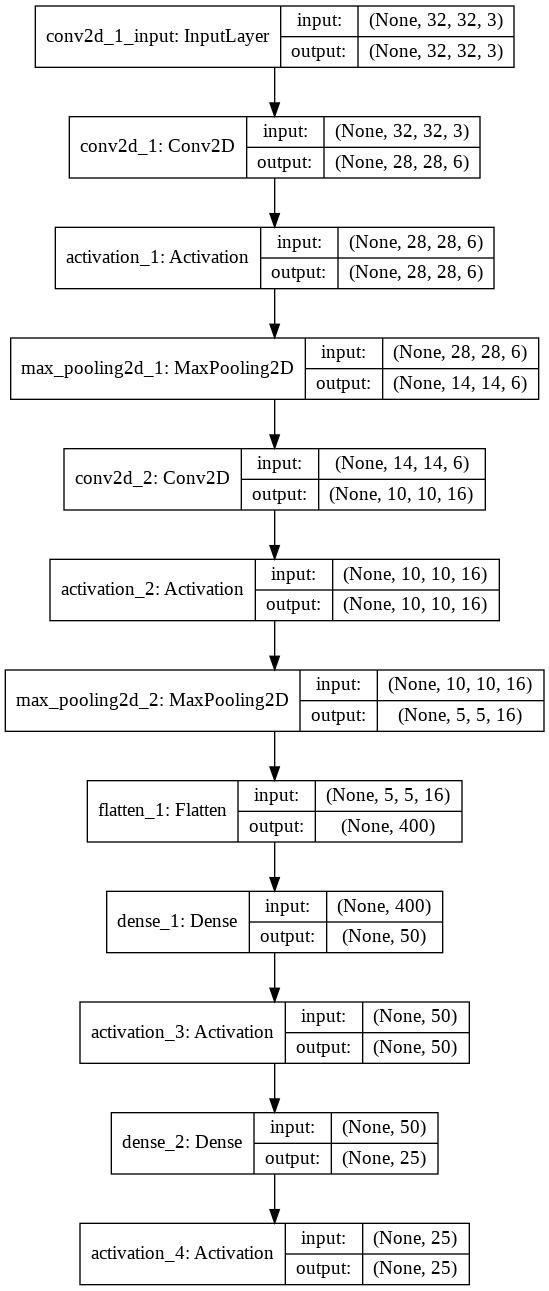
\includegraphics[scale=0.28]{img/base-model.png}
  \caption{Esquema que representa el modelo \textit{BaseNet}.}
  \label{fig:base-model}
\end{figure}

Aquí es donde podemos ver mejor la estructura del modelo. Se puede ver de forma más clara que antes la estructua secuencial
que tiene, además de cada una de las capas y de los tamaños de las entradas y de las salidas de éstas.

Teniendo el modelo ya construido y compilado, para hacernos una idea de como de bueno es, podemos entrenarlo y probarlo
con el conjunto de test. Es muy importante, antes de empezar, guardar los pesos que tiene el modelo. De esta forma, podremos
restablecerlos posteriormente, para poder reentrenar el modelo. Para guardar los pesos, podemos hacerlo de la siguiente
forma:

\begin{lstlisting}
# Guardar los pesos iniciales del modelo
weights = model.get_weights()
\end{lstlisting}

Ahora ya podemos proceder al entrenamiento. Es muy importante destacar que, con los datos de entrenamiento de los que disponemos,
solo se tiene que entrenar con el 90\% de éstos; el 10\% restante se tiene que dejar para validar el modelo, y de esta forma poder
obtener unas gráficas para el error y la \textit{accuracy} en los conjuntos de entrenamiento y de validación. Estos
valores que se obtienen para el conjunto de validación son, en general, una buena aproximación de lo que se puede obtener
en el conjunto de test, si la muestra es lo suficientemente representativa de la población total, claro está.

Para entrenar el modelo, lo hacemos de la siguiente forma:

\begin{lstlisting}
# Entrenar el modelo
history = model.fit(
    x_train,
    y_train,
    validation_split=0.1,
    epochs=epochs,
    batch_size=batch_size,
    verbose=1
)
\end{lstlisting}

Especificamos que se utilizan las particiones de entrenamiento $x\_train$ (las imágenes) e $y\_train$ (la etiqueta asociada
a cada una de las imágenes del conjunto de entrenamiento). Además, con $validation\_split = 0.1$ indicamos que solo el
10\% de los datos se utilizarán para validar el modelo. Se especifica también el tamaño del \textit{batch} (recordemos que
lo habíamos fijado a 32) y el número de épocas (30 inicialmente). El parámetro $verbose$ es solo para mostrar el progreso
del entrenamiento; no tiene ningún otro fin.

Este método devuelve una historia, la cuál se almacena en la variable $history$. Esta historia contiene trazas de la evolución
de los valores de la función de pérdida y de \textit{accuracy} en los conjuntos de entrenamiento y de validación.
Para este caso, hemos obtenido los siguientes resultados:

\begin{figure}[H]
  \centering
  \begin{subfigure}[t]{0.5\textwidth}
    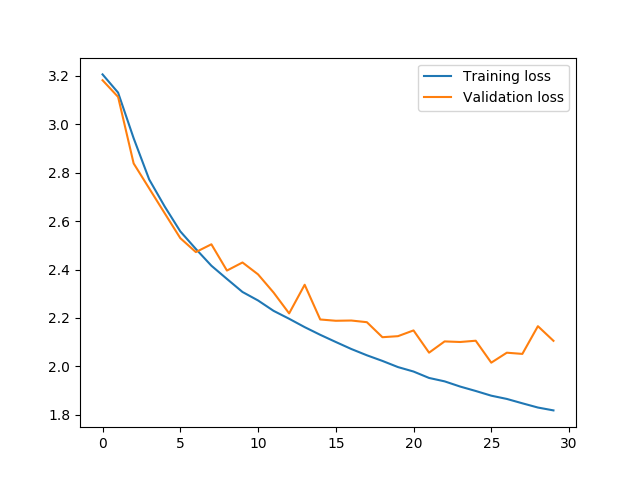
\includegraphics[scale=0.42]{img/base-model-loss.png}
    \caption{Evolución de la función de pérdida.}
    \label{fig:base-model-loss}
  \end{subfigure}%
  ~ \quad
  \begin{subfigure}[t]{0.5\textwidth}
    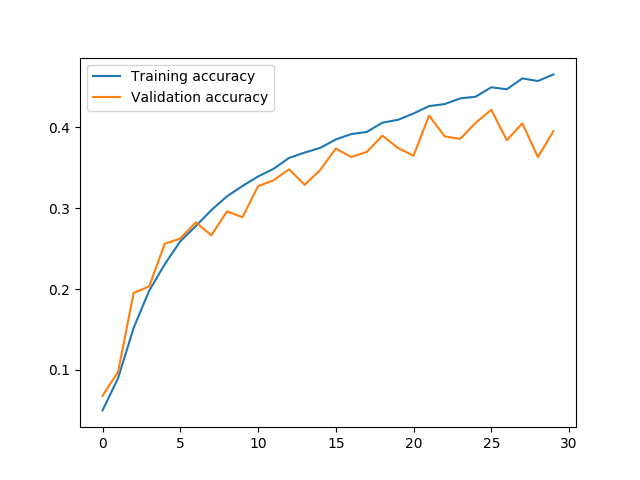
\includegraphics[scale=0.42]{img/base-model-acc.png}
    \caption{Evolución de la \textit{accuracy}.}
    \label{fig:base-model-acc}
  \end{subfigure}
  \caption{Historia del modelo \textit{BaseNet}.}
  \label{fig:basenet-history}
\end{figure}

Podemos ver que no se produce \textit{overfit}, ya que a medida que el valor del error o de la función de pérdida va
bajando en el conjunto de entrenamiento, también lo hace en el de validación, hasta que llega a las últimas épocas, donde dicho
valor se queda más o menos se queda un poco por encima del de entrenamiento, pareciendo que se estanca.
En ningún momento el error en validación llega a subir. Si esto hubiese sucedido, podríamos haber afirmado de forma clara
que se ha producido \textit{overfit} en nuestro modelo. Si miramos también la \textit{accuracy}, podemos ver que, a medida
que va subiendo dicho valor en el conjunto de entrenamiento, también lo hace en el de validación.
Aquí de nuevo sucede algo como en el caso de la función de pérdida, ya que parece que en las últimas épocas este valor se va
quedando un poco estancado, aunque no dista mucho del valor obtenido en el conjunto de entrenamiento.

Sin embargo, aunque el modelo no padezca de \textit{overfit}, sí que lo hace de \textit{underfit}: la evolución de los valores
de la función de pérdida y de la \textit{accuracy}, aunque en un principio parecen buenos ya que el error va disminuyendo y la
precisión aumentando, no es del todo satisfactoria. Podemos ver claramente como el error, aún en el conjunto de entrenamiento,
sigue siendo bastante alto (en las últimas épocas se queda en torno a $1.8$, valor bastante alto), y en el caso de la
precisión se queda en torno a $0.45$. En el caso del conjunto de validación, aunque al principio los valores sean más o
menos parejos con el conjunto de entrenamiento en ambas gráficas, podemos ver como al cabo de aproximadamente unas 15-20 épocas
los valores empiezan a ser dispares. En el caso de la función de pérdida, al final, los valores que se obtienen están en torno a 2,
mientras que en la precisión los valores obtenidos no superan el $0.4$, quedándose por debajo de los obtenidos en entrenamiento.

En líneas generales, estos resultados son demasiado pobres: lo ideal hubiese sido alcanzar un error cercano a 1 o
más bajo y una precisión superior a 0.5 en el conjunto de entrenamiento, y que los valores obtenidos en el conjunto de
validación hubiesen seguido casi perfectamente a los de entrenamiento. Por tanto, de aquí podemos extraer que todavía
existe mucho margen de mejora.

Es importante destacar, antes de continuar, que todos los resultados que se obtienen dependen de la ejecución. Es decir,
que para dos ejecuciones puede que los resultados no sean exactamente los mismos; sin embargo, podemos decir que estarán
bastante cerca, en general, ya que los datos son los mismos.

Para tener una idea de cómo de bien funciona nuestro modelo base con el conjunto de test, y para tener un valor de
\textit{accuracy} que podemos utilizar para comparar este modelo base con las mejoras futuras, vamos a hacer que prediga
las etiquetas del conjunto $x\_test$ (las imágenes de test), y compararemos dichos valores con los reales, los cuáles están
en la variable $y\_test$. Para hacer dicha predición, podemos hacerla de la siguiente forma:

\begin{lstlisting}
# Predecir los datos
prediction = model.predict(
    x_test,
    batch_size=batch_size,
    verbose=1
)
\end{lstlisting}

De esta forma, especificamos que el modelo prediga las etiquetas asociadas al conjunto $x\_test$ y se le especifica un tamaño
de \textit{batch}, que será el número de elementos máximos que se predigan de golpe; es decir, no se va mandar a CPU/GPU un
conjunto de datos de mayor tamaño que el especificado. El parámetro $verbose$ es, de nuevo, para mostrar el proceso.

El valor de \textit{accuracy} comparando los valores predichos con los reales gira en torno a $0.4$ tras realizar
algunas pruebas. Dicho valor, a pesar de no ser del todo horrible para un modelo tan simple, es bastante bajo, y creemos
que tiene cierto margen de mejora. ya que posiblemente, con realizar algunas modificaciones, podamos llegar una \textit{accuracy}
igual o superior a $0.5$. Por tanto, vamos a intentar mejorar nuestro modelo en la próxma sección,
para ver hasta dónde somos capaces de llegar.

\section{\textsc{Mejora del modelo}}

En esta sección, vamos a ir proponiendo una serie de mejoras que podemos hacer sobre el modelo. Estas mejoras son acumulativas,
es decir, que se van realizando una sobre la otra, siempre y cuando ofrezcan unos buenos resultados.

Para cada caso, vamos a discutir brevemente qué es lo que se va a mejorar, qué parámetros se van a utilizar y cuáles son los
resultados obtenidos. Para cada experimento mostraremos gráficas, iguál que las que se pueden ver en la figura
\ref{fig:basenet-history}.

Una vez que hayamos encontrado un modelo bueno (es decir, uno que no sufre ni de \textit{overfit} ni de \textit{underfit}, y
ofrece unos valores de error y precisión razonables en el conjunto de validación), utilizaremos el conjunto de test para
ver cómo de bien lo hace, y es entonces cuando podremos comparar dichos resultados con el modelo base, para poder ver hasta
dónde hemos llegado. En ningún otro caso utilizaremos dicho conjunto, ya que no es buena idea dejarnos llevar por los resultados
obtenidos en test para decir que un modelo es mejor que otro; para eso tenemos el conjunto de validación.

\subsection{Normalización de los datos}

La primera mejora que vamos a introducir es la normalización de los datos de entrada, haciendo que éstos tengan media
$\mu = 0$ y desviación típica $\sigma = 1$. Se introduce esta mejora porque se sabe que gracias a la normalización se pueden
obtener unos mejores resultados, además de que el entrenamiento de la red se puede llegar a acelerar.

La manera más fácil de normalizar los datos es utilizar un generador de la clase $ImageDataGenerator$. Para crearlo, podemos
utilizar el siguiente fragmento de código:

\begin{lstlisting}
datagen_train = ImageDataGenerator(
    featurewise_center=True,
    featurewise_std_normalization=True,
    validation_split=0.1
)
\end{lstlisting}

De esta forma, creamos un generador para los datos de entrenamiento, el cuál hará que la media sea 0 (con el parámetro
$featurewise\_center = True$), normalizará la desviación típica (con el parámetro $featurewise\_std\_normalization = True$)
y creará una partición de validación con el 10\% de los datos de entrenamiento (parámetro $validation\_split = 0.1$).

Como el generador utiliza normalización, hace falta entrenarlo con los datos de entrenamiento. Esto lo podemos hacer
de la siguiente forma:

\begin{lstlisting}
# Entrenar generadores
datagen_train.fit(x_train)
\end{lstlisting}

Con el generador ya entrenado, podemos obtener los iteradores que se van a utilizar a la hora de entrenar el modelo. Habrá
un iterador para el conjunto de entrenamiento y otro para el conjunto de validación. Obtener estos iteradores se puede
hacer de la siguiente forma:

\begin{lstlisting}
# Crear flow de entrenamiento y validacion
train_iter = datagen_train.flow(
    x_train,
    y_train,
    batch_size=batch_size,
    subset='training'
)

validation_iter = datagen_train.flow(
    x_train,
    y_train,
    batch_size=batch_size,
    subset='validation'
)
\end{lstlisting}

En el primer caso, creamos un iterador de entrenamiento, utilizando para ello los datos de $x\_train$ e $y\_train$. Es aquí
donde especificamos el tamaño del \textit{batch} (recordemos que se ha establecido que sea 32), y se indica que los datos
pertenecen al subconjunto de \textit{training} (esto es porque se ha especificado en el generador que se utilice
$validation\_split = 0.1$). Para el conjunto de validación el proceso es casi igual, solo que el subconjunto del que
se extraerán los datos es \textit{validation}.

Es importane destacar que a la hora de crear los iteradores (al llamar a los métodos $flow$), los
datos son barajados (por defecto el parámetro $shuffle$ está puesto a \textbf{True}). Esto es importante, ya que si no,
Keras solo cogería el primer 10\% de los datos como validación, lo cuál puede hacer que el conjunto de validación no represente
para nada al conjunto de entrenamiento, y por tanto, los resultados obtenidos en validación sean pésimos.

Una vez hecho esto. ya podemos entrenar el modelo. Como en este caso utilizamos generadores, no podemos utilizar el
método $fit()$ tal y como hicimos anteriormente, si no que tendremos que utilizar el método $fit\_generator()$. El entrenamiento
que se ha realizado se puede ver en el siguiente fragmento de código:

\begin{lstlisting}
history = model.fit_generator(
    train_iter,
    steps_per_epoch=len(x_train)*0.9/batch_size,
    epochs=epochs,
    validation_data=validation_iter,
    validation_steps=len(x_train)*0.1/batch_size
)
\end{lstlisting}

Especificamos que para entrenar se va a utilizar el iterador $train\_iter$ creado anteriormente. Por cada época se van a
realizar $len(x\_train)*0.9/batch\_size$ pasos (esto es, del tamaño del conjunto de entrenamiento original se cogerá el
90\% de dicho tamaño, que representa el porcentaje de datos que se utilizarán para entrenar, y este número de elementos
se dividirá entre el tamaño del \textit{batch}, que es 32; de esta forma se sabe cuántos pasos hay que dar para el tamaño de
\textit{batch} especificado). Luego se indica cuántas épocas se quieren entrenar (de momento, viendo los resultados que se han
obtenido en el apartado anterior, vamos a conservar su valor anterior, que es 35, ya que no se produce un \textit{overfit} que
nos indique que haga falta rebajar dicho número). Se indica que como datos de validación se va a utilizar el $validation\_iter$
creado anteriormente y se indica el número de pasos que se van a hacer a la hora de validar, lo cuál se hace de forma similar
a cómo se hizo con el conjunto de entrenamiento, solo que se utilizará el 10\% del tamaño del conjunto de entrenamiento.

Con el entrenamiento ya hecho, vamos a estudiar las gráficas para ver qué tal ha ido:

\begin{figure}[H]
  \centering
  \begin{subfigure}{.5\textwidth}
    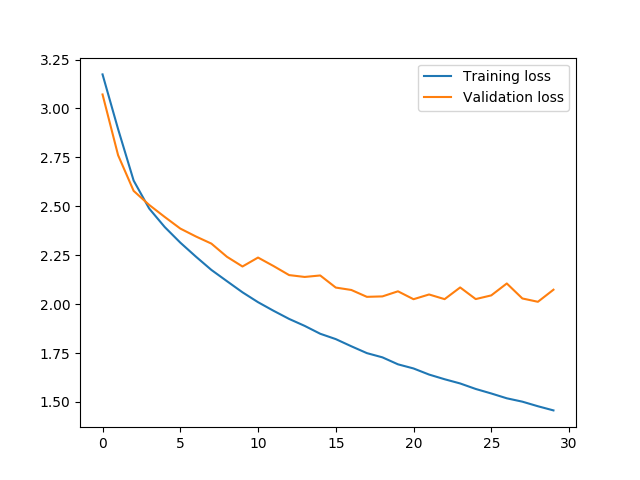
\includegraphics[scale=0.4]{img/norm-loss.png}
    \subcaption{Evolución de la función de pérdida.}
    \label{fig:norm-loss}
  \end{subfigure}%
  ~ \quad
  \begin{subfigure}{.5\textwidth}
  	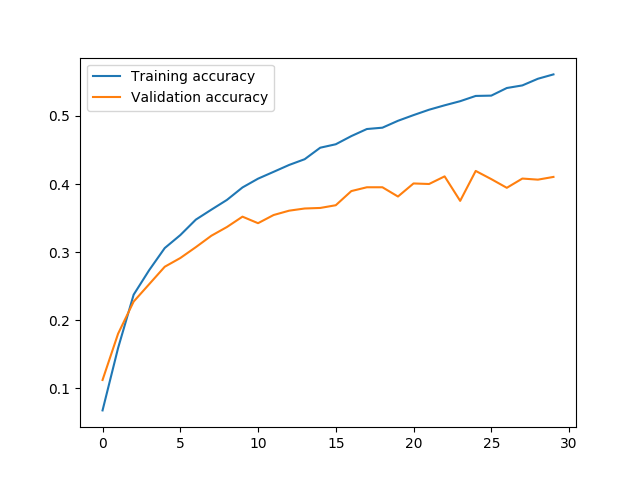
\includegraphics[scale=0.4]{img/norm-acc.png}
  	\subcaption{Evolución de la \textit{accuracy}.}
  	\label{fig:norm-acc}
  \end{subfigure}
  \caption{Historia del modelo \textit{BaseNet} con normalización.}
  \label{fig:norm-history}
\end{figure}

Como podemos ver, comparando los resultados con los que se pueden ver en la figura \ref{fig:basenet-history} los valores de
pérdida son menores en el conjunto de entrenamiento que los que teníamos anteriormente. Además, el valor de \textit{accuracy}
es más alto que el que habíamos obtenido en el caso anterior para el el conjunto de entrenamiento. Sin embargo, si estudiamos
los resultados obtenidos en validación, vemos que no ha habido ninguna mejora significativa, ya que los resultados son bastante
parecidos a los que teníamos anteriormente.

Además de eso, si estudiamos los valores de entrenamiento y de validación de forma conjunta, podemos ver que, a diferencia
de lo que sucedía en la figura \ref{fig:basenet-history}, aquí los resultados en validación se quedan mucho más cortos cuando
llegamos a las últimas épocas. Al principio, los valores van bastante pegados, pero a medida que aumentan el número de épocas,
éstos se van despegando, hasta llegar al resultado final que podemos ver en las gráfias de la figura \ref{fig:norm-history}.

En líneas generales podemos ver que los valores de la función de pérdida en validación se quedan bastante por encima de los de
entrenamiento, y la \textit{accuracy} se queda bastante por debajo de la de entrenamiento. Aparte, en ambos parece que se estanca
en las últimas épocas, mientras que los valores obtenidos en entrenamiento siguen mejorando. Por tanto, podemos detectar cierto
\textit{overfit}, ya que aunque se mejore en entrenamiento, no hay mejoras reales en validación, con lo cuál parece
que el modelo está comenzando a memorizar los datos de entrenamiento. Posiblemente, de haber entrenado algunas épocas más,
los valores de validación hubiesen empezado a empeorar.

Tras este breve análisis podemos ver que, a pesar de que normalizar ha permitido mejorar los resultados obtenidos en entrenamiento,
los de validación aún se quedan muy cortos. Por tanto, ha habido cierta mejora, pero no significativa. Esto puede deberse a que
solo se normaliza la entrada, y a media que se van haciendo convoluciones, dicha normalización se pierde. Con lo cuál, parece
lógico que se tengan que introducir capas de normalización en la red para que los datos siempre estén normalizados, aunque
esto lo haremos más adelante. De momento, conservaremos la normalización, ya que es una mejora que siempre ayuda y, si conseguimos
combinarla con alguna otra mejora, puede que los resultados sean bastante mejores.

\subsection{Aumento de datos}

La siguiente mejora que podemos probar es el aumento de datos. De esta forma, a partir de los datos que tenemos para entrenar
el modelo, podemos generar nuevos datos aplicándoles transformaciones, como por ejemplo rotaciones, zoom, espejo, etc. Para
estudiar si existe mejora al aplicar esta técnica, vamos a probar una serie de transformaciones que utilizaremos en combinación
con la normalización, ya que siempre es útil normalizar los datos de entrada. Las transformaciones a probar son las siguientes:

\begin{itemize}
  \item \textbf{\textit{Flip} horizontal}. Este aumento consiste en voltear la imagen en el eje horizontal. Puede ser
  una mejora interesante debido a que va a invertir la imagen, y por ende los elementos de la imagen, con lo cuál podemos llegar
  a tener la imagen normal en alguna de las épocas de entrenamiento, y la imagen volteada en otra, la cuál será tratada como una
  nueva   muestra de entrenamiento. Por tanto, es posible que ayude a generalizar mejor.
  \item \textbf{Zoom}. Este aumento consiste en realizar un zoom sobre la imagen, tanto para alejarse de ella como para
  acercarse. Podría ser interesante aplicar este aumento ya que nos podría ofrecer información sobre una misma imagen a distintas
  escalas, desde más cerca o más lejos por ejemplo.
  \item \textbf{Rotación}. Este aumento rota la imagen en $\alpha$ grados en cualquiera de los dos sentidos. Es un aumento que puede
  ser útil cuando la imagen no ha sido tomada en condiciones óptimas (por ejemplo, con algún tipo de rotación, haciendo que los
  objetos estén de lado). De esta forma, se puede aprender más mirando un mismo objeto con distintas orientaciones.
  \item \textbf{\textit{Flip} horizontal + zoom}. Esta es una mejora que combina tanto el \textit{flip} com el zoom, con
  el objetivo de ver si al invertir la imagen y hacer zoom se puede aprender más, y por tanto, generalizar mejor, ya que se
  tienen nuevos elementos en el conjunto de entrenamiento a distintas esclas.
\end{itemize}

Ya que en este apartado vamos a generar nuevas imágenes, podemos probar a aumentar el número de épocas de 35 a 50, ya que con
pocas épocas no se va a notar nada el aumento. Esto se debe a que los aumentos se generan sobre la marcha, y tienen una probabilidad
de aparecer o no. Con lo cuál, podría darse la mala suerte de que no salgan muchos aumentos en pocas épocas, y entonces es
como si estuviésemos entrenando con los datos normales. Además, así podremos ver si al insertar nuevos datos y aumentar
el número de épocas, podemos disminuir un poco el \textit{overfit} que se producía, tal y como se puede ver en la figura
\ref{fig:norm-history}.

Antes de ver los resultados que ofrece cada uno de estos aumentos, hace falta conocer cómo se hacen los aumentos.
Gracias a la clase $ImageDataGeneratos$ podemos hacerlo de forma bastante sencilla, ya que podemos especificar qué
aumentos queremos hacer (recordemos que también vamos a especificar que se normalicen los datos y que vamos a crear
una partición de validación).

Para especificar que queremos hacer un \textbf{\textit{flip} horizontal}, además de aplicar normalización y crear
un conjunto de validación, podemos hacerlos de la siguiente forma:

\begin{lstlisting}
# Datagen con flip horizontal
datagen_train_flip = ImageDataGenerator(
    featurewise_center=True,
    featurewise_std_normalization=True,
    validation_split=0.1,
    horizontal_flip=True
)
\end{lstlisting}

Lo único diferente a lo que hacíamos anteriormente es especificar el parámetro $horizontal\_flip$ poniéndolo a \textbf{True}.

Podemos declarar un generador con \textbf{zoom} de la siguiente forma:

\begin{lstlisting}
# Datagen con zoom de 0.2
datagen_train_zoom = ImageDataGenerator(
    featurewise_center=True,
    featurewise_std_normalization=True,
    validation_split=0.1,
    zoom_range=0.2
)
\end{lstlisting}

El parámetro $zoom\_range$ controla la escala del zoom, tanto para alejarse como para acercarse de la imagen. En este caso,
se ha especificado que dicho valor sea 0.2, un valor no muy grande y que es comunmente.

Para declarar un generador que utilice \textbf{rotación}, podemos utilizar algo como lo que se ve a continuación:

\begin{lstlisting}
# Datagen con rotacion de 25
datagen_train_rot = ImageDataGenerator(
    featurewise_center=True,
    featurewise_std_normalization=True,
    validation_split=0.1,
    rotation_range=25
)
\end{lstlisting}

La rotación se especifica con el parámetro $rotation\_range$. En este caso, se ha especificado que se rote como máximo
$25º$ en cualquiera de los dos sentidos. Se ha escogido este valor porque se cree que es razonable que se realicen pequeñas
rotaciones sobre la imagen en vez de rotaciones muy abruptas.

Finalmente, podemos crear un generador que combine \textbf{\textit{flip} horizontal} junto con \textbf{zoom} de la
siguiente forma:

\begin{lstlisting}
# Datagen con flip horizontal y zoom de 0.2
datagen_train_fz = ImageDataGenerator(
    featurewise_center=True,
    featurewise_std_normalization=True,
    validation_split=0.1,
    horizontal_flip=True,
    zoom_range=0.2
)
\end{lstlisting}

Aquí no hay nada nuevo que comentar, ya que es una combinación de dos de los generadores vistos anteriormente.

Para utilizar los generadores, de nuevo tenemos que utilizar el método $fit()$ tal y como hicimos antes, además de crear
los iteradores correspondientes. Para entrenar el modelo, de nuevo podemos utilizar el método $fit\_generator()$.

Una vez comentados los aspectos generales, vamos a analizar los resultados obtenidos para cada tipo de aumento de datos,
comparándolos con lo que teníamos anteriormente y entre ellos, y decidiendo cuál es el mejor para este problema.

\begin{figure}[H]
  \centering
  \begin{subfigure}{.5\textwidth}
    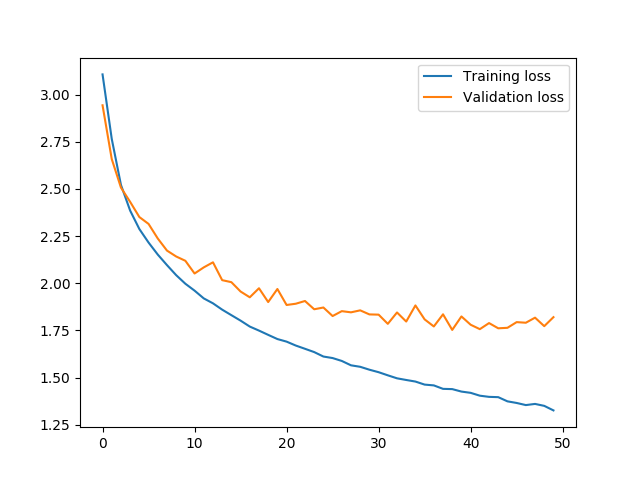
\includegraphics[scale=0.4]{img/aug-flip-loss.png}
    \subcaption{Evolución de la función de pérdida.}
    \label{fig:aug-flip-loss}
  \end{subfigure}%
  ~ \quad
  \begin{subfigure}{.5\textwidth}
    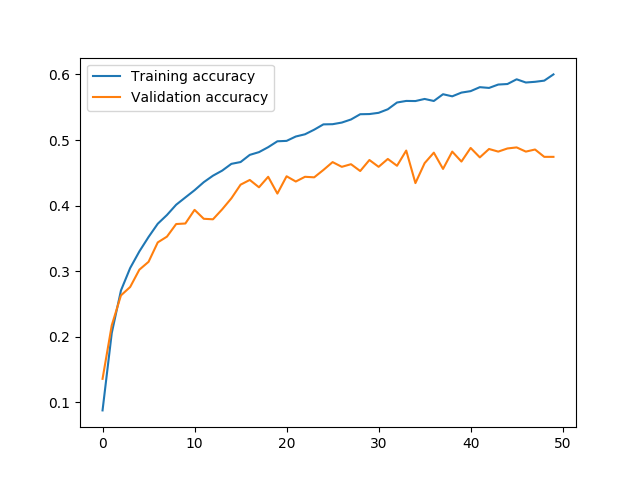
\includegraphics[scale=0.4]{img/aug-flip-acc.png}
    \subcaption{Evolución de la \textit{accuracy}.}
    \label{fig:aug-flip-acc}
  \end{subfigure}
  \caption{Historia del aumento de datos con \textit{flip} horizontal.}
  \label{fig:history-aug-flip}
\end{figure}

\begin{figure}[H]
  \begin{subfigure}{.5\textwidth}
    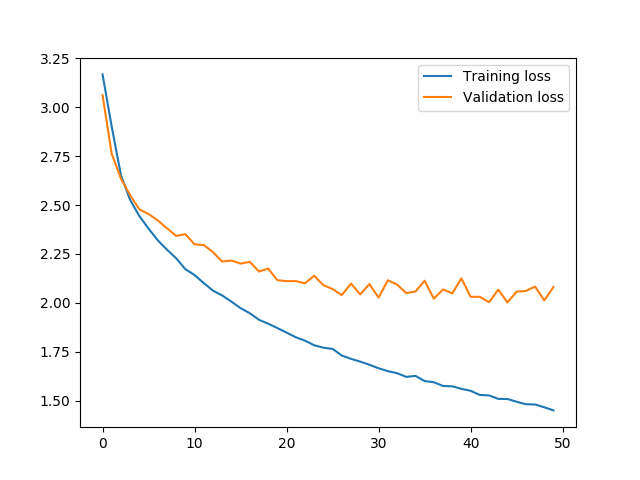
\includegraphics[scale=0.4]{img/aug-zoom-loss.png}
    \subcaption{Evolución de la función de pérdida.}
    \label{fig:aug-zoom-loss}
  \end{subfigure}%
  ~ \quad
  \begin{subfigure}{.5\textwidth}
    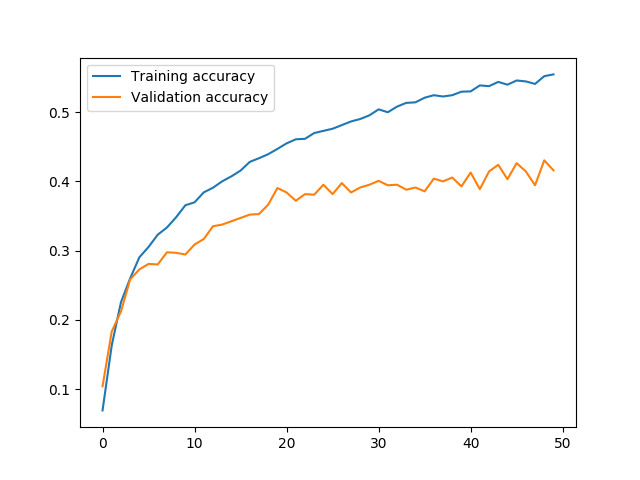
\includegraphics[scale=0.4]{img/aug-zoom-acc.png}
    \subcaption{Evolución de la \textit{accuracy}.}
    \label{fig:aug-zoom-acc}
  \end{subfigure}
  \caption{Historia del aumento de datos con zoom.}
  \label{fig:history-aug-zoom}
\end{figure}

\begin{figure}[H]
  \begin{subfigure}{.5\textwidth}
    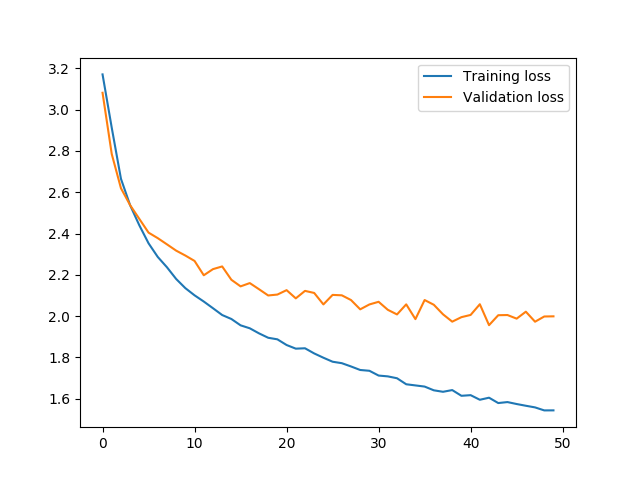
\includegraphics[scale=0.4]{img/aug-rot-loss.png}
    \subcaption{Evolución de la función de pérdida.}
    \label{fig:aug-rot-loss}
  \end{subfigure}%
  ~ \quad
  \begin{subfigure}{.5\textwidth}
    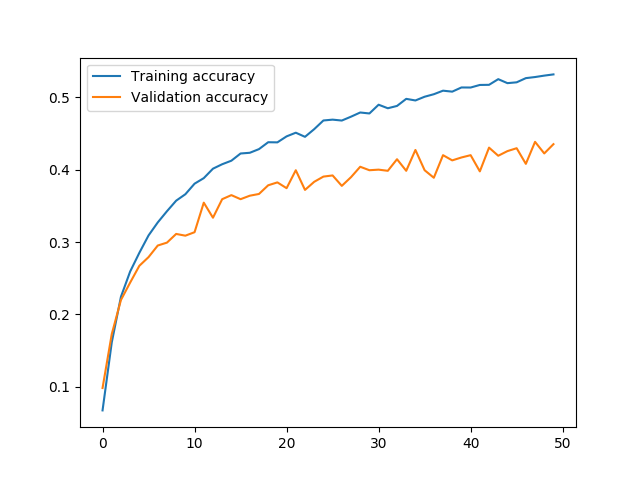
\includegraphics[scale=0.4]{img/aug-rot-acc.png}
    \subcaption{Evolución de la \textit{accuracy}.}
    \label{fig:aug-rot-acc}
  \end{subfigure}
  \caption{Historia del aumento de datos con rotación.}
  \label{fig:history-aug-rot}
\end{figure}

\begin{figure}[H]
  \begin{subfigure}{.5\textwidth}
    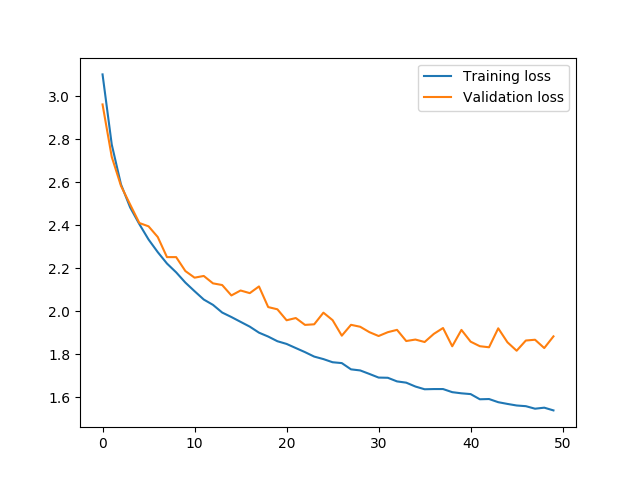
\includegraphics[scale=0.4]{img/aug-flipzoom-loss.png}
    \subcaption{Evolución de la función de pérdida.}
    \label{fig:aug-flipzoom-loss}
  \end{subfigure}%
  ~ \quad
  \begin{subfigure}{.5\textwidth}
    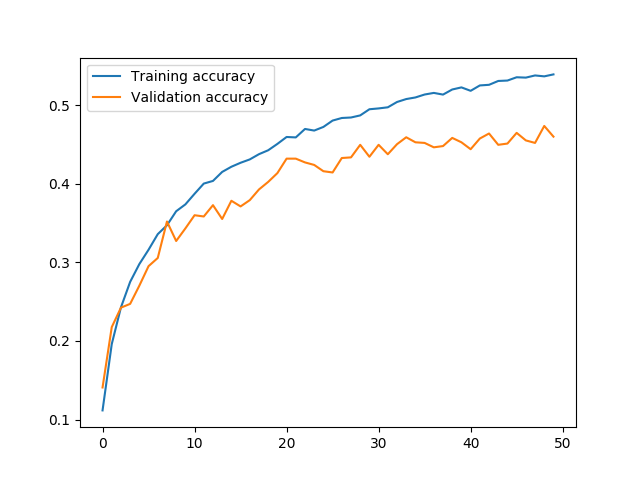
\includegraphics[scale=0.4]{img/aug-flipzoom-acc.png}
    \subcaption{Evolución de la \textit{accuracy}.}
    \label{fig:aug-flipzoom-acc}
  \end{subfigure}
  \caption{Historia del aumento de datos con \textit{flip} horizontal y zoom.}
  \label{fig:history-aug-flipzoom}
\end{figure}

En general, si miramos los resultados, podemos ver que hay aumentos de datos, como por ejemplo el zoom y la rotación
que no aportan casi ninguna mejora, ya que los resultados obtenidos para entrenamiento son bastante buenos, mientras
que en validación se queda bastante corto, tanto en las gráficas de error como en la de \textit{accuracy}. El error
en validación se queda, en ambos casos, muy cerca de 2, mientras que el de entrenamiento baja hasta 1.5-1.6. La
\textit{accuracy} en validación se queda en torno a 0.4 en validación, mientras que en entrenamiento supera los
0.5 en ambos casos. Estos resultados recuerdan mucho a los que se pueden ver en la figura \ref{fig:norm-history}, y por
tanto, no representan una mejora suficiente como para volver a utilizarlos en el futuro.

En cambio, si comparamos los resultados obtenidos para los casos en los que se utiliza \textit{flip} horizontal, vemos
que sí que se produce cierta mejora respecto a los modelos anteriores, y a los otros modelos con aumentos de zoom y rotación.
En los dos modelos que se usa el \textit{flip} horizontal el error en validación se sitúa por debajo de 2, mejorando por tanto 
los resultados obtenidos por el modelo base y por el modelo con solo la normalización. La \textit{accuracy} en validación
también ha sufrido un ligero incremento, situándose en ambos casos por encima de 0.4. Por tanto, el modelo mejora ciertamente
al utilizar \textit{flip} horizontal.

Ahora bien, si comparamos ambos modelos, vemos que en el caso en el que solo se hace el \textit{flip}, los valores en
validación son un poco mejores que los obtenidos al aumentar los datos con \textit{flip} y zoom. Sin embargo, en este
segundo caso, los resultados de validación se quedan más cerca de los de entrenamiento. Por tanto, en el segundo caso,
se podría decir que se está generalizando mejor, a pesar de que los resultados son, en general, un poco peores. A pesar
de eso, parece que en ambos modelos las curvas de validación se van a estancar en unas pocas épocas más, mientras
que las de entrenamiento continuarán mejorando. Por tanto, ninguno de los dos modelos está libre de potencial
\textit{overfit}.

Si nos basamos en como de bien se puede generalizar, la opción clara, de momento, sería escoger como mejor aumento
de datos el que realiza un \textit{flip} junto con un zoom. Sin embargo, si nos atendemos a los resultados obtenidos
en validación, el mejor es el que hace solo el \textit{flip}. Como el modelo puede ser regularizado para reducir
el \textit{overfit}, vamos a escoger como \textbf{mejor aumento} el que \textbf{solo realiza un \textit{flip} horizontal}
por habernos ofrecido unos mejores resultados en validación.

\subsection{Aumento de la profundidad de la red}

La siguiente mejora que nos podemos plantear es aumentar la profundidad de la red. Para ello, se van a proponer dos
arquitecturas. Ambas se compararán, y se elegirá la mejor. En un principio, ambas se compararán solo con la normalización,
y después se mirará como son afectadas por el aumento de datos con \textit{flip} horizontal (el aumento que mejores resultados
ha proporcionado).

Ambos modelos están compuestos por dos módulos convolucionales, cada uno con dos capas convolucionales, y una capa
de \textit{max pooling} al final. Además, en ambos modelos se ha pasado a tener 3 capas totalmente conectadas, formando
una red de $128 \times 50 \times 25$ neuronas que se encargarán de clasificar según la información extraída por la red
convolucional, y en los dos modelos el número de canales va creciendo a medida que se van haciendo convoluciones.
Al tener una arquitectura como esta, no se reduce el tamaño de las imágenes tan rápidamente como pasaba antes,
ya que antes de cada \textit{max pool} hay dos convoluciones en vez de una.

A pesar de las similitudes que tienen los dos modelos, existen dos diferencia importante entre ellos: el tamaño del
\textit{kernel} de las convoluciones y el número de canales de salida:

\begin{itemize}
  \item En el caso de la primera red, el primer módulo convolucional está compuesto por dos convoluciones $5 \times 5$, con
  8 y 16 canales de salida, respectivamente. El segundo módulo está compuesto por dos capas convolucionales con \textit{kernel}
  de tamaño $3 \times 3$, y con 32 y 64 canales de salida.
  \item En la segunda red los dos módulos utilizan convoluciones de tamaño $3 \times 3$, y el número de canales es 16 y 32 para
  el primer módulo convolucional y de 64 y 64 para el segundo módulo.
\end{itemize}

En el primer modelo, las convoluciones del primer módulo se han hecho así para imitar las que hace \textit{BaseNet}, solo
que se ha cambiado el número de canales de salida de la primera convolución. Las del segundo módulo tienen un tamaño
de $3 \times 3$ para no reducir demasiado la imagen, además de que las convoluciones de este tamaño son más rápidas
que las $5 \times 5$. El número de canales de salida es siempre una potencia de 2. No hay ningún motivo para que
sea un número potencia de 2, ya que la red no va a obtener mejores resultados por tener canales de salida de tamaño
potencia de 2.

En el segundo modelo, todas las convoluciones son de $3 \times 3$ porque son menos costosas desde el punto de vista
computacional. Todos los canales de salida de las capas convolucionales son, de nuevo, potencias de 2. Sin embargo,
a diferencia del modelo anterior, el número de canales de la primera capa convoluciona es de 16, y se incrementa
hasta un máximo de 64, ya que se cree que no tiene sentido hacer canales más grandes debido a que éstos pueden
llevar a un \textit{overfit} excesivo sin regularizar.

Una vez que hemos comentado los aspectos generales de ambas arquitecturas, vamos a ver cómo sería la implementación
de ellas. El código correspondiente al primer modelo es el siguiente:

\begin{lstlisting}
# Definicion del nuevo modelo
model_v2 = Sequential()
model_v2.add(Conv2D(8, kernel_size=(5, 5), padding='valid', input_shape=input_shape))
model_v2.add(Activation('relu'))
model_v2.add(Conv2D(16, kernel_size=(5, 5), padding='valid'))
model_v2.add(Activation('relu'))
model_v2.add(MaxPooling2D(pool_size=(2, 2)))

model_v2.add(Conv2D(32, kernel_size=(3, 3), padding='valid'))
model_v2.add(Activation('relu'))
model_v2.add(Conv2D(64, kernel_size=(3, 3), padding='valid'))
model_v2.add(Activation('relu'))
model_v2.add(MaxPooling2D(pool_size=(2, 2)))

model_v2.add(Flatten())
model_v2.add(Dense(units=128))
model_v2.add(Activation('relu'))
model_v2.add(Dense(units=50))
model_v2.add(Activation('relu'))
model_v2.add(Dense(units=25))
model_v2.add(Activation('softmax'))
\end{lstlisting}

El segundo modelo se ha declarado de la siguiente forma:

\begin{lstlisting}
# Definicion del nuevo modelo
model_v3 = Sequential()
model_v3.add(Conv2D(16, kernel_size=(3, 3), padding='valid', input_shape=input_shape))
model_v3.add(Activation('relu'))
model_v3.add(Conv2D(32, kernel_size=(3, 3), padding='valid'))
model_v3.add(Activation('relu'))
model_v3.add(MaxPooling2D(pool_size=(2, 2)))

model_v3.add(Conv2D(64, kernel_size=(3, 3), padding='valid'))
model_v3.add(Activation('relu'))
model_v3.add(Conv2D(64, kernel_size=(3, 3), padding='valid'))
model_v3.add(Activation('relu'))
model_v3.add(MaxPooling2D(pool_size=(2, 2)))

model_v3.add(Flatten())
model_v3.add(Dense(units=128))
model_v3.add(Activation('relu'))
model_v3.add(Dense(units=50))
model_v3.add(Activation('relu'))
model_v3.add(Dense(units=25))
model_v3.add(Activation('softmax'))
\end{lstlisting}

Una vez compilados los modelos, vamos a entrenarlos y a ver los resultados que obtenemos. Es importante destacar que, para entrenar
estos modelos, el número de épocas ha sido reducido 35. De esta forma, si los modelos tardan más en entrenarse, no se realizan
tantas épocas, y por tanto el tiempo de entrenamiento es menor. Además, como vimos en la sección anterior, al haber entrenado 50
épocas, los modelos estaban muy cerca de padecer de sobreajuste, con lo cuál parece sensato reducir el número de épocas para
intentar evitar que esto suceda para estos nuevos modelos.

Otra cosa importante a destacar es que primero se entrenarán los modelos utilizando solo la normalización. Posteriormente,
si todo va bien, entrenaremos con aumento de datos, aplicando un \textit{flip} horizontal sobre las imágenes, y miraremos si
existe mejora.

Una vez comentado estos detalles, vamos a pasar a estudiar los resultados obtenidos.

\begin{figure}[H]
  \centering
  \begin{subfigure}{.5\textwidth}
    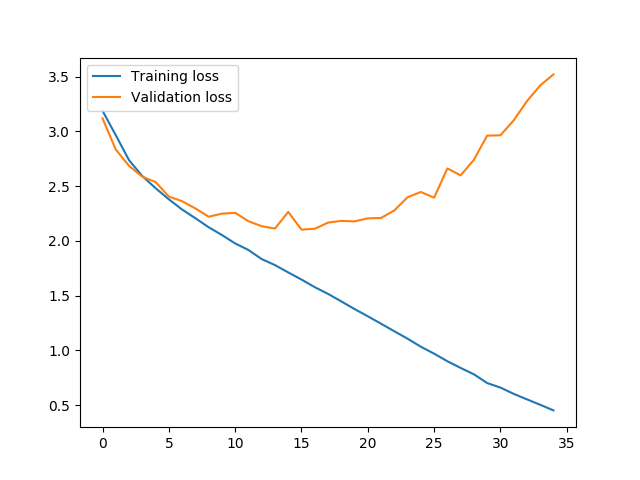
\includegraphics[scale=0.4]{img/deep1-nodrop-loss.png}
    \subcaption{Evolución de la función de pérdida.}
    \label{fig:deep1-nodrop-loss}
  \end{subfigure}%
  ~ \quad
  \begin{subfigure}{.5\textwidth}
    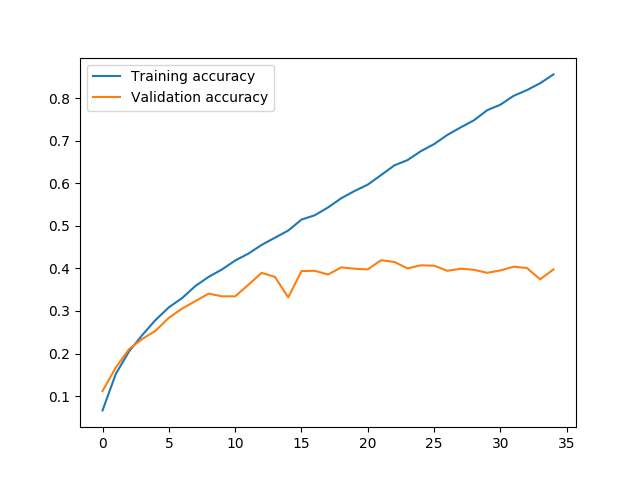
\includegraphics[scale=0.4]{img/deep1-nodrop-acc.png}
    \subcaption{Evolución de la \textit{accuracy}.}
    \label{fig:deep1-nodrop-acc}
  \end{subfigure}
  \caption{Historia del primer modelo profundo.}
  \label{fig:history-deep1-nodrop}
\end{figure}

\begin{figure}[H]
  \centering
  \begin{subfigure}{.5\textwidth}
    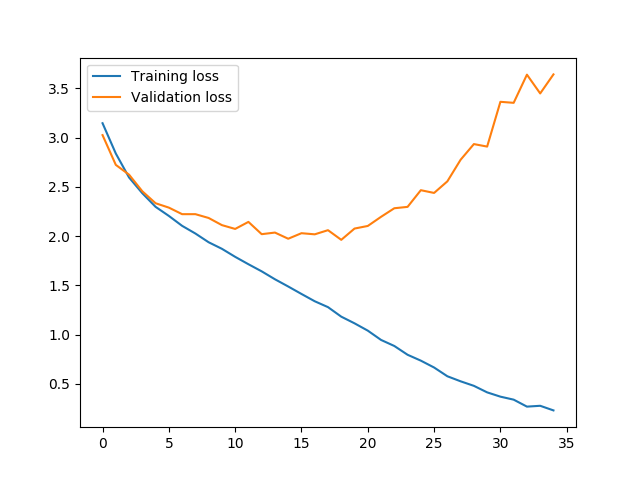
\includegraphics[scale=0.4]{img/deep2-nodrop-loss.png}
    \subcaption{Evolución de la función de pérdida.}
    \label{fig:deep2-nodrop-loss}
  \end{subfigure}%
  ~ \quad
  \begin{subfigure}{.5\textwidth}
    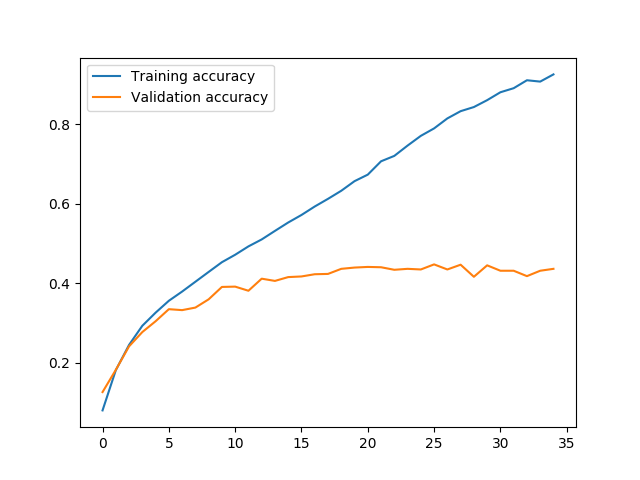
\includegraphics[scale=0.4]{img/deep2-nodrop-acc.png}
    \subcaption{Evolución de la \textit{accuracy}.}
    \label{fig:deep2-nodrop-acc}
  \end{subfigure}
  \caption{Historia del segundo modelo profundo.}
  \label{fig:history-deep2-nodrop}
\end{figure}

Se puede observar a simple vista que los resultados obtenidos son muy malos. En ambos casos, el \textit{overfit} es
evidente, ya que los valores del error en validación empiezan a subir a partir de las 15 épocas, mientras que los valores
del error en entrenamiento sigue constante. Esto también se refleja en las gráficas de \textit{accuracy}, donde podemos
ver que la precisión en el conjunto de entrenamiento va mejorando, mientras que la del conjunto de validación se queda
estancada y no mejora nada. Toda esta situación llevará a que la red no sea capaz de generalizar correctamente, ya que al
existir sobreajuste, la red acaba memorizando los datos de entrenamiento, y obtendrá unos resultados pésimos con nuevos
datos que nunca antes ha visto.

Este problema se debe a que hemos aumentado la profundidad de la red, y con eso, el número de parámetros de la red.
Estos parámetros pueden tomar cualquier valor, ya que no hay ninguna restricción sobre ellos.
Cuando sucede esto, los parámetros se pueden ``descontrolar'', tomando valores que le permiten ajustarse
más a los datos de entrenamiento, y por tanto, disminuir el error en el conjunto de entrenamiento, ya que es lo que
se está intentando minimizar. Esto nos llevará a unos resultados como los que podemos ver en las figuras
\ref{fig:history-deep1-nodrop} y \ref{fig:history-deep2-nodrop}, donde los resultados en el conjunto de entrenamiento
son muy buenos mientras que los de validación son muy malos.

Este problema puede ser difícil de solventar, ya que no hay una única manera de intentar reducir el \textit{overfit}.
Una idea simple sería aplicar \textit{early stopping}, parando el entrenamiento antes de que empiece a sobreajustar.
En este caso, sería parar el entrenamiento alrededor de las 10-15 épocas. Sin embargo, si hacemos eso, el modelo que
obtendremos será bastante malo, ya que no habrá aprendido lo suficiente debido a que los valores del error y la precisión
serán bastante malos en general (como podemos ver en las gráficas). Por tanto, para solventar este problema podemos probar
a utilizar una técnica de regularización como \textbf{Dropout}, la cuál procederemos a ver a continuación.

\subsection{Mejora extra: regularización mediante Dropout}

La forma más sencilla de regularizar nuestros modelos es el \textbf{Dropout}. Este proceso consiste en escoger una proporción
de las neuronas de una capa de forma aleatoria y en desactivar las conexiones de dichas neuronas con las neuronas
de la capa siguiente, de forma que no participan en el proceso. Luego, a la hora de predecir, no se realiza Dropout, ya
que participan todas las conexiones. En cambio, los valores predichos son ponderados en función del número de veces que
esa conexión se haya dejado activa. Está demostrado que, en general, este proceso ayuda a reducir el \textit{overfit},
y por tanto, hace que la red sea capaz de generalizar mejor. Sin embargo, como cualquier método de regularización,
hace falta usarlo con cuidado, ya que insertar demasiadas capas de Dropout puede llevar a una regularización excesiva
del modelo, y por tanto, que el modelo sufra de \textit{underfitting}, ya que los valores que pueden tomar los parámetros
se habrán limitado en exceso.

Para regularizar nuestros modelos, vamos a insertar una capa de Dropout después de cada módulo convolucional (recordemos que
un módulo está formado por un conjunto de capas \textbf{Convolución-Convolución-Max Pooling}). No existe como tal una regla de
oro que nos diga dónde insertar las capas de Dropout, ya que eso depende mucho del modelo. En este caso se ha decidido
poner una capa de Dropout al final de cada módulo convolucional porque se considera que el sobreajuste viene a raíz de pasar
de un módulo convolucional a otro debido a que al final de uno se reduce la imagen a la mitad, y al principio del siguiente
se aplican convoluciones para extraer características. Al tener imagenes tan pequeñas en general, los tamaños se reducen muy
rápido, con lo cual, al tener convoluciones que producen salidas bastante grandes, se empiezan a extraer
características muy particulares de dichas imágenes, lo que al final provoca que se acaben memorizando los datos de entrenamiento.
Al regularizar no se deja que se entrenen todos los parámetros de la red a la vez, sino solo una parte. De esta forma,
se llega a evitar el problema comentado anteriormente.

Cuando insertemos capas de Dropout, hace falta especificar la proporción de conexiones que vamos a desactivar. En algunos
artículos se aconseja que si se utiliza Dropout en la red convolucional (no en las capas totalmente conectadas) que
la proporción de conexiones que se desactiven sea pequeña \cite{inproceedings}. Por tanto, siendo $p$ la proporción
de conexiones a desactivar, vamos a hacer que $p = 0.2$. De esta forma, estamos desactivando un número de conexiones
pequeño, pero aún así suficiente para regularizar la red.

Con esto comentado, vamos a ver cómo quedarían los dos modelos anteriores aplicando Dropout. El código que define
la arquitectura del primer modelo, al que llamaremos \textit{Modelo A}, se puede ver a continuación:

\begin{lstlisting}
# Definicion del nuevo modelo
model_v2 = Sequential()
model_v2.add(Conv2D(8, kernel_size=(5, 5), padding='valid', input_shape=input_shape))
model_v2.add(Activation('relu'))
model_v2.add(Conv2D(16, kernel_size=(5, 5), padding='valid'))
model_v2.add(Activation('relu'))
model_v2.add(MaxPooling2D(pool_size=(2, 2)))
model_v2.add(Dropout(0.2))

model_v2.add(Conv2D(32, kernel_size=(3, 3), padding='valid'))
model_v2.add(Activation('relu'))
model_v2.add(Conv2D(64, kernel_size=(3, 3), padding='valid'))
model_v2.add(Activation('relu'))
model_v2.add(MaxPooling2D(pool_size=(2, 2)))
model_v2.add(Dropout(0.5))

model_v2.add(Flatten())
model_v2.add(Dense(units=128))
model_v2.add(Activation('relu'))
model_v2.add(Dense(units=50))
model_v2.add(Activation('relu'))
model_v2.add(Dense(units=25))
model_v2.add(Activation('softmax'))
\end{lstlisting}

El segundo modelo, al que llamaremos \textit{Modelo B}, introduciendo regularización, se puede representar de la siguiente manera:

\begin{lstlisting}
# Definicion del nuevo modelo
model_v3 = Sequential()
model_v3.add(Conv2D(16, kernel_size=(3, 3), padding='valid', input_shape=input_shape))
model_v3.add(Activation('relu'))
model_v3.add(Conv2D(32, kernel_size=(3, 3), padding='valid'))
model_v3.add(Activation('relu'))
model_v3.add(MaxPooling2D(pool_size=(2, 2)))
model_v3.add(Dropout(0.2))

model_v3.add(Conv2D(64, kernel_size=(3, 3), padding='valid'))
model_v3.add(Activation('relu'))
model_v3.add(Conv2D(64, kernel_size=(3, 3), padding='valid'))
model_v3.add(Activation('relu'))
model_v3.add(MaxPooling2D(pool_size=(2, 2)))
model_v3.add(Dropout(0.5))

model_v3.add(Flatten())
model_v3.add(Dense(units=128))
model_v3.add(Activation('relu'))
model_v3.add(Dense(units=50))
model_v3.add(Activation('relu'))
model_v3.add(Dense(units=25))
model_v3.add(Activation('softmax'))
\end{lstlisting}

Estos modelos tienen que ser compilados y entrenados de la misma forma que hemos visto antes. Utilizaremos de nuevo 35 épocas,
para comparar si ha habido mejora al utilizar regularización respecto a los resultados que hemos obtenido anteriormente. De nuevo,
de momento solo utilizaremos normalización al utilizar los generadores. Si existe mejora, probaremos a utilizar el generador
que utiliza aumento de datos de \textit{flip} horizontal.

A continuación podemos ver las gráficas obtenidas para ambos modelos:

\begin{figure}[H]
  \centering
  \begin{subfigure}{.5\textwidth}
    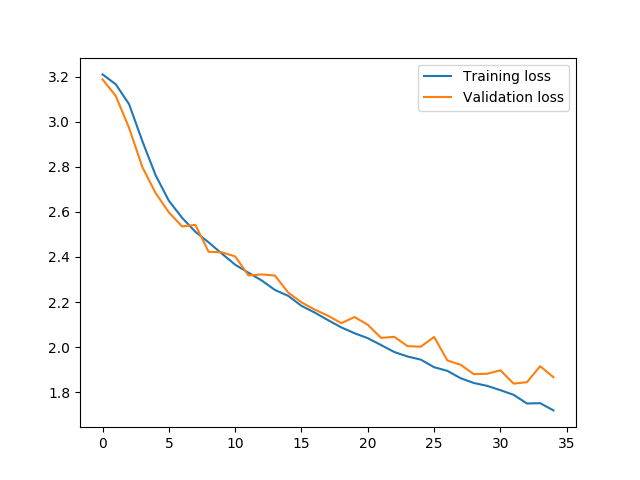
\includegraphics[scale=0.4]{img/deep1-drop-loss-35.png}
    \subcaption{Evolución de la función de pérdida.}
    \label{fig:deep1-drop-loss-35}
  \end{subfigure}%
  ~ \quad
  \begin{subfigure}{.5\textwidth}
    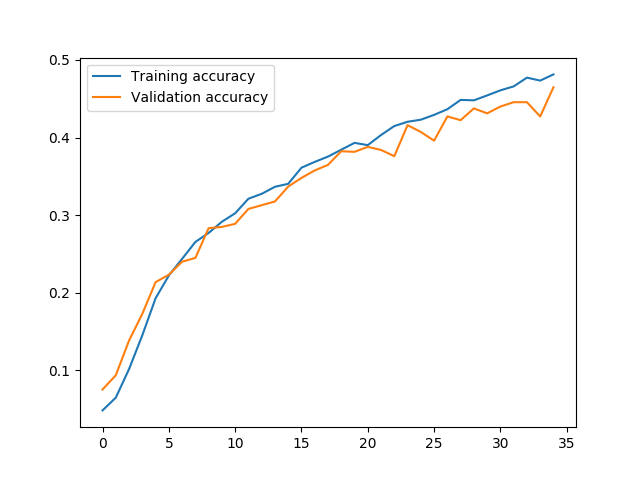
\includegraphics[scale=0.4]{img/deep1-drop-acc-35.png}
    \subcaption{Evolución de la \textit{accuracy}.}
    \label{fig:deep1-drop-acc-35}
  \end{subfigure}
  \caption{Historia del \textit{Modelo A}.}
  \label{fig:history-deep1-drop-35}
\end{figure}

\begin{figure}[H]
  \centering
  \begin{subfigure}{.5\textwidth}
    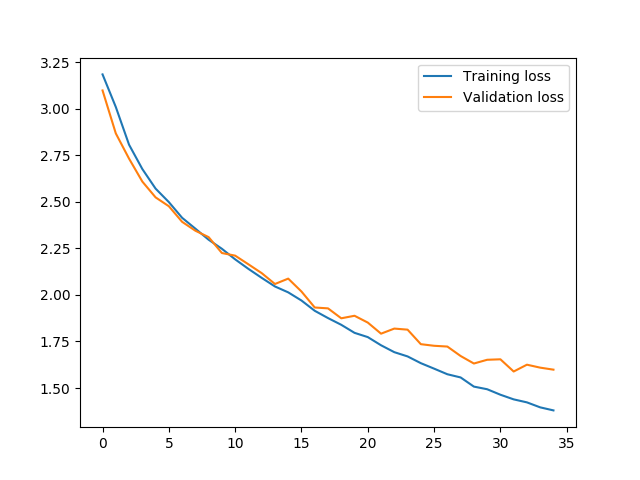
\includegraphics[scale=0.4]{img/deep2-drop-loss-35.png}
    \subcaption{Evolución de la función de pérdida.}
    \label{fig:deep2-drop-loss-35}
  \end{subfigure}%
  ~ \quad
  \begin{subfigure}{.5\textwidth}
    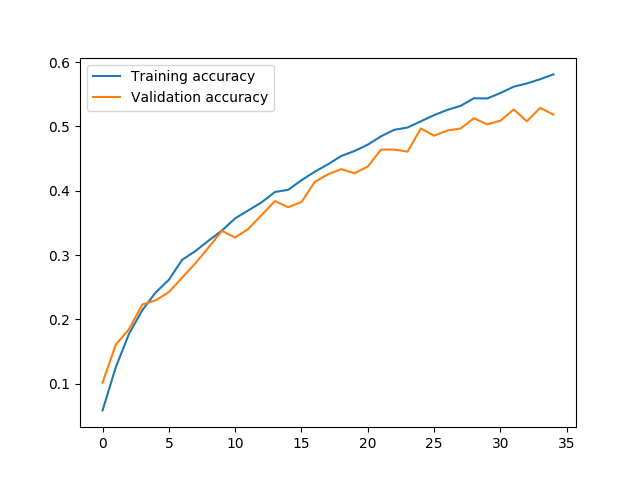
\includegraphics[scale=0.4]{img/deep2-drop-acc-35.png}
    \subcaption{Evolución de la \textit{accuracy}.}
    \label{fig:deep2-drop-acc-35}
  \end{subfigure}
  \caption{Historia del \textit{Modelo B}.}
  \label{fig:history-deep2-drop-35}
\end{figure}

Si comparamos estas gráficas con las figuras \ref{fig:history-deep1-nodrop} y \ref{fig:history-deep2-nodrop}, podemos ver
que los modelos han mejorado un montón. Ahora en ambos los resultados obtenidos en validación se parecen mucho más a los
de entrenamiento, ya que en ambos casos, las curvas van más pegadas. Además, se ha eliminado completamente el \textit{overfit},
ya que los resultados obtenidos en validación van mejorando a medida que los de entrenamiento mejoran. Podemos ver
claramente que en las gráficas de la evolución del error no se produce un incremento en validación en las últimas épocas,
cosa que sí que sucedía en los casos anteriores.

Ahora, si analizamos los resultados, podemos ver que en general son muy buenos. El error en ambos casos se sitúa por debajo
de 2, y la precisión está por encima de 0.4, tal y como pasaba con los resultados que se pueden ver en la figura
\ref{fig:history-aug-flip}, aunque en este caso son mejores, ya que no hay sobreajuste. En general, los resultados obtenidos
por el \textit{Modelo B} en validación son mejores debido a que el error en validación es menor y la \textit{accuracy} es
mayor. Además, los valores obtenidos para el conjunto de entrenamiento son bastante parejos, y son bastante mejores que
los obtenidos en el \textit{Modelo A}.

Ya que los resultados obtenidos con 35 épocas han sido bastante buenos, vamos a subir de nuevo el número de épocas a 50,
para ver si se pueden mantener al entrenar los modelos durante más épocas. Que suceda esto sería lo ideal, ya que, al entrenar
más, podríamos tener un modelo que generalice mejor, siempre y cuando los resultados obtenidos en validación sigan
el mismo comportamiento que los obtenidos anteriormente.

Por tanto, restablecemos los pesos de los modelos y los entrenamos de nuevo. Los resultados obtenidos se pueden
ver a continuación:

\begin{figure}[H]
  \centering
  \begin{subfigure}{.5\textwidth}
    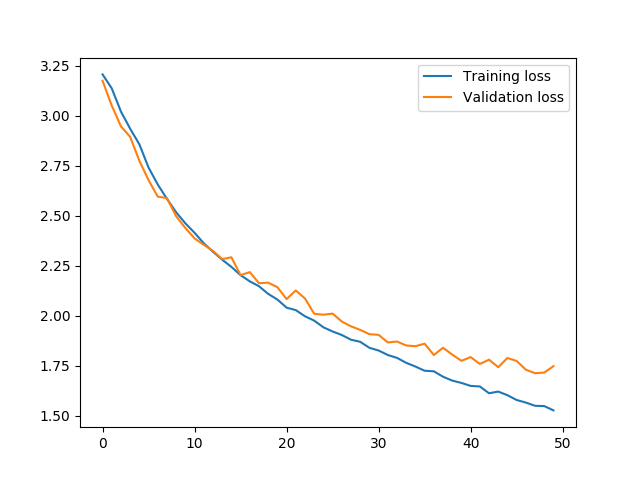
\includegraphics[scale=0.4]{img/deep1-drop-loss-50.png}
    \subcaption{Evolución de la función de pérdida.}
    \label{fig:deep1-drop-loss-50}
  \end{subfigure}%
  ~ \quad
  \begin{subfigure}{.5\textwidth}
    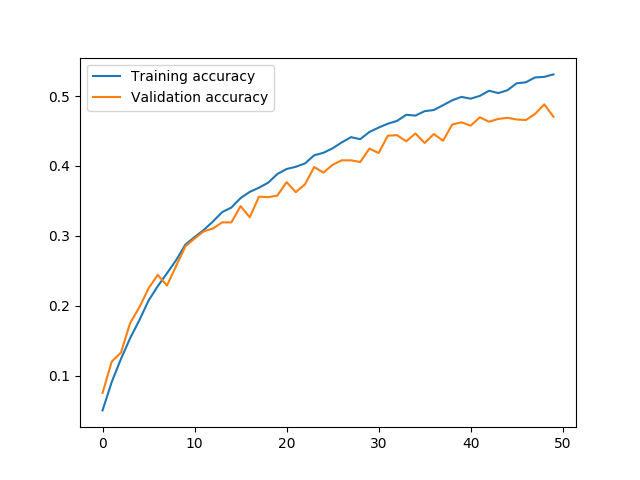
\includegraphics[scale=0.4]{img/deep1-drop-acc-50.png}
    \subcaption{Evolución de la \textit{accuracy}.}
    \label{fig:deep1-drop-acc-50}
  \end{subfigure}
  \caption{Historia del \textit{Modelo A}.}
  \label{fig:history-deep1-drop-50}
\end{figure}

\begin{figure}[H]
  \centering
  \begin{subfigure}{.5\textwidth}
    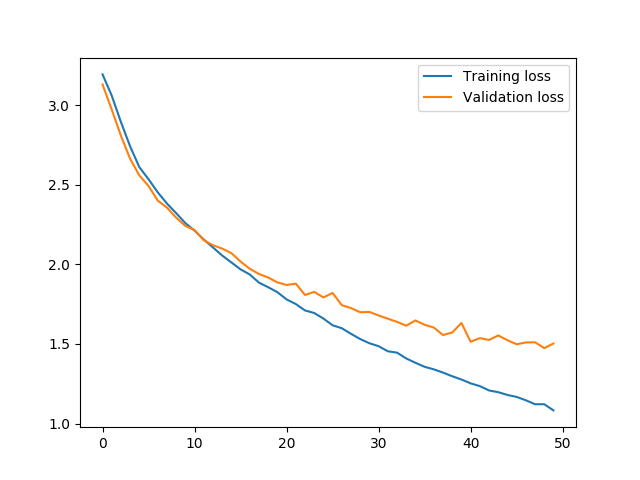
\includegraphics[scale=0.4]{img/deep2-drop-loss-50.png}
    \subcaption{Evolución de la función de pérdida.}
    \label{fig:deep2-drop-loss-50}
  \end{subfigure}%
  ~ \quad
  \begin{subfigure}{.5\textwidth}
    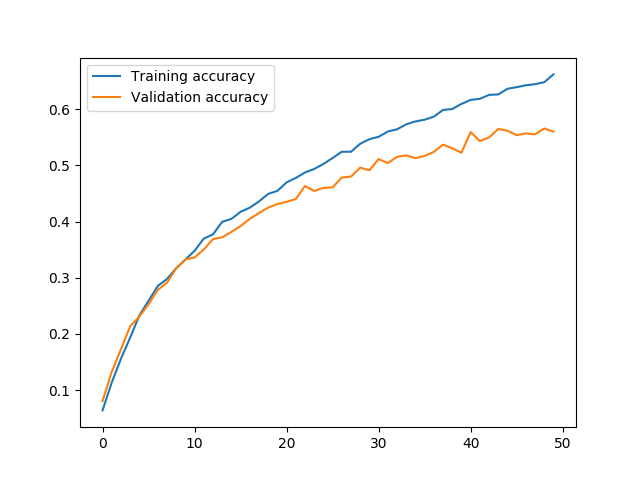
\includegraphics[scale=0.4]{img/deep2-drop-acc-50.png}
    \subcaption{Evolución de la \textit{accuracy}.}
    \label{fig:deep2-drop-acc-50}
  \end{subfigure}
  \caption{Historia del \textit{Modelo B}.}
  \label{fig:history-deep2-drop-50}
\end{figure}

Podemos ver que, en general, al haber aumentado el número de épocas, los valores de validación
han mejorado en ambos modelos tanto para los valores de la función de pérdida como para la
\textit{accuracy}. En general, para el \textit{Modelo A}, los resultados obtenidos en validación
están más pegados a los valores de entrenamiento que los obtenidos en el \textit{Modelo B}. No
obstante, los obtenidos en el \textit{Modelo B} son mucho mejores que los obtenidos en el
\textit{Modelo A}, tanto en validación como en entrenamiento. Es en este modelo donde, por primera
vez, se consigue una \textit{accuracy} en validación superior al 0.5, lo cuál son buenas noticias,
ya que hemos conseguido mejorar bastante el modelo base, el cuál no llegaba ni al 0.4, tal y como
se puede ver en la figura \ref{fig:basenet-history}. Así que, en general, aumentar el número de
épocas ha sido una buena idea.

Para elegir el mejor modelo, vamos a probar a entrenar ambos modelos con aumento de datos, para ver
cuál se comporta mejor. Las gráficas obtenidas son las siguientes:

\begin{figure}[H]
  \centering
  \begin{subfigure}{.5\textwidth}
    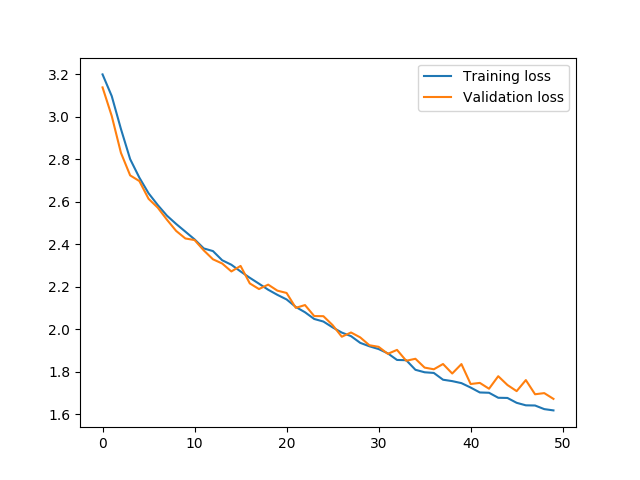
\includegraphics[scale=0.38]{img/deep1-aug-loss.png}
    \subcaption{Evolución de la función de pérdida.}
    \label{fig:deep1-aug-loss}
  \end{subfigure}%
  ~ \quad
  \begin{subfigure}{.5\textwidth}
    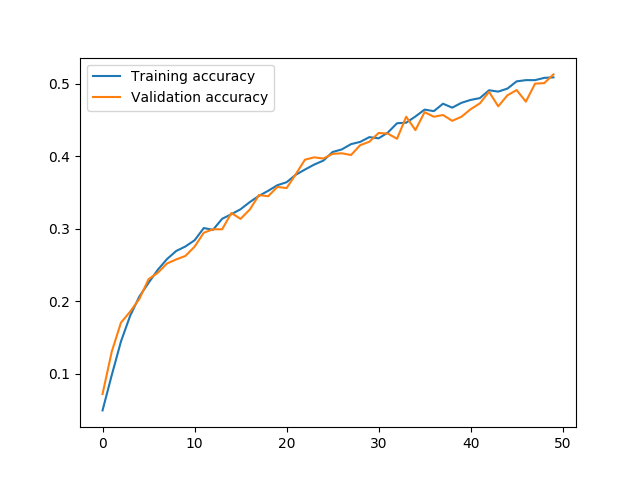
\includegraphics[scale=0.38]{img/deep1-aug-acc.png}
    \subcaption{Evolución de la \textit{accuracy}.}
    \label{fig:deep1-aug-acc}
  \end{subfigure}
  \caption{Historia del \textit{Modelo A}.}
  \label{fig:deep1-aug}
\end{figure}

\begin{figure}[H]
  \centering
  \begin{subfigure}{.5\textwidth}
    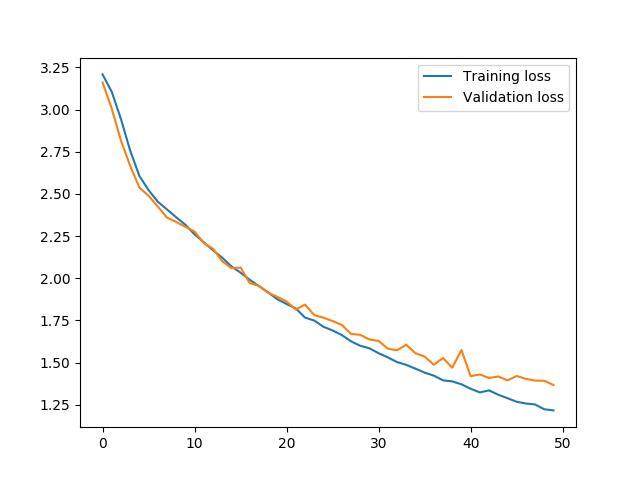
\includegraphics[scale=0.4]{img/deep2-aug-loss.png}
    \subcaption{Evolución de la función de pérdida.}
    \label{fig:deep2-aug-loss}
  \end{subfigure}%
  ~ \quad
  \begin{subfigure}{.5\textwidth}
    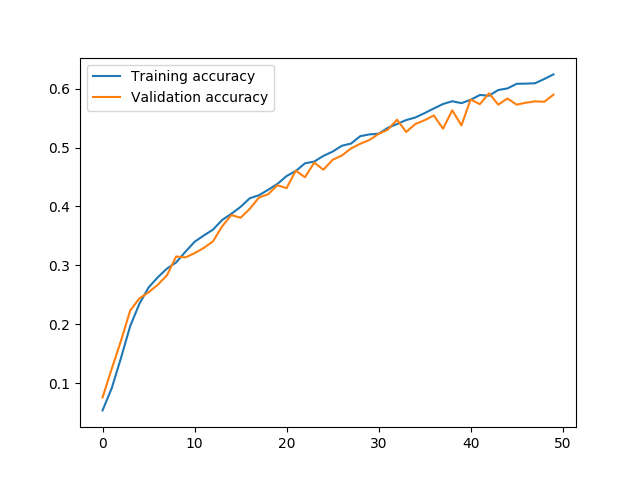
\includegraphics[scale=0.4]{img/deep2-aug-acc.png}
    \subcaption{Evolución de la \textit{accuracy}.}
    \label{fig:deep2-aug-acc}
  \end{subfigure}
  \caption{Historia del \textit{Modelo B}.}
  \label{fig:deep2-aug}
\end{figure}

En ambos casos los resultados son muy buenos, siendo incluso mejores que los que obtuvimos
utilizando solo la normalización. Podemos ver aquí cómo los resultados obtenidos en el conjunto
de validación en ambos modelos se ajustan mejor a los obtenidos en entrenamiento que antes. Además,
en este caso, la \textit{accuracy} obtenida con el \textit{Modelo A} en las últimas épocas llega al
0.5, superando a la que tenía anteriormente. Por tanto, introducir aumento de datos ha mejorado
significativamente los resultados obtenidos en el \textit{Modelo A}.

En el caso del \textit{Modelo B}, podemos ver como el error en validación se ve reducido más aún,
y la \textit{accuracy} comienza a acercarse a 0.6. Además, el error obtenido en este caso es bastante
menor que el del \textit{Modelo A}. Si observamos el error en entrenamiento, podemos ver que en este
caso es mayor que el que se ve en la figua \ref{fig:history-deep2-drop-50}, aunque esto no nos preocupa
mucho, ya que en validación obtiene mejores resultados.

Por tanto, como veredicto final, vamos a quedarnos con el \textit{Modelo B}, ya que es el que ha
obtenido unos mejores resultados en el conjunto de validación y, además, no presenta \textit{overfit}.
Por tanto, hemos conseguido crear una arquitectura más profunda que es capaz de conseguir unos buenos
resultados y que, de momento, parece que es capaz de generalizar bastante bien. Veremos si con la
próxima mejora somos capaces de sacar el máximo potencial al modelo.

\subsection{Capas de normalización}

La última mejora que queremos introducir en el modelo es la \textit{Batch Normalization} o normalización
por lotes. Esto es, se introducen algunas capas en la red que se encargan de aprender valores con
los cuáles pueden transformar los datos para intentar normalizarlos. Esta es una técnica que permite
regularizar la red, reducir los tiempos de entrenamiento y obtener unos resultados mejores en general.

Se ha decidido insertar una capa de normalización después de cada capa convolucional y de cada
capa totalmente conectada. De esta forma, después de cada operación, los datos serán normalizados,
con lo cuál no se perderá esa normalización que se hace sobre los datos de entrada. Además, se cree
que el rendimiento de la red mejorará al utilizar una normalización después de cada convolucional y
totalmente conectada. Si en las gráficas se ve que se produce \textit{underfitting} porque a lo mejor
se ha regularizado demasiado, se reducirá el número de capas de normalización. No obstante, en un principio,
se cree que el impacto será más bien positivo, y que permitirá a la red generalizar mejor. El único
lugar donde no se pondrá normalización es después de la capa de \textit{softmax} ya que no tiene sentido
(esta capa es la salida de la red, y da probabilidades; por tanto, no tiene sentido utilizar normalización
ahí).

El problema de introducir normalización viene a la hora de determinar dónde ponerla, si antes o después de
la función de activación. Para ello, vamos a construir dos modelos: uno primero al que llamaremos
\textit{Modelo Pre}, donde la normalización estará antes de la función de activación; y un segundo modelo
al que llamaremos \textit{Modelo Post}, en el que la capa de normalización estará justo después de la función
de activación.

El \textit{Modelo Pre} se define de la siguiente forma:

\begin{lstlisting}
# Definicion del nuevo modelo
model_batch_pre = Sequential()
model_batch_pre.add(Conv2D(16, kernel_size=(3, 3), padding='valid', input_shape=input_shape))
model_batch_pre.add(BatchNormalization())
model_batch_pre.add(Activation('relu'))
model_batch_pre.add(Conv2D(32, kernel_size=(3, 3), padding='valid'))
model_batch_pre.add(BatchNormalization())
model_batch_pre.add(Activation('relu'))
model_batch_pre.add(MaxPooling2D(pool_size=(2, 2)))
model_batch_pre.add(Dropout(0.2))

model_batch_pre.add(Conv2D(64, kernel_size=(3, 3), padding='valid'))
model_batch_pre.add(BatchNormalization())
model_batch_pre.add(Activation('relu'))
model_batch_pre.add(Conv2D(64, kernel_size=(3, 3), padding='valid'))
model_batch_pre.add(BatchNormalization())
model_batch_pre.add(Activation('relu'))
model_batch_pre.add(MaxPooling2D(pool_size=(2, 2)))
model_batch_pre.add(Dropout(0.5))

model_batch_pre.add(Flatten())
model_batch_pre.add(Dense(units=128))
model_batch_pre.add(BatchNormalization())
model_batch_pre.add(Activation('relu'))
model_batch_pre.add(Dense(units=50))
model_batch_pre.add(BatchNormalization())
model_batch_pre.add(Activation('relu'))
model_batch_pre.add(Dense(units=25))
model_batch_pre.add(Activation('softmax'))
\end{lstlisting}

La arquitectura del \textit{Modelo Post} viene definida por el siguiente código:

\begin{lstlisting}
# Definicion del nuevo modelo
model_batch_post = Sequential()
model_batch_post.add(Conv2D(16, kernel_size=(3, 3), padding='valid',
							input_shape=input_shape))
model_batch_post.add(Activation('relu'))
model_batch_post.add(BatchNormalization())
model_batch_post.add(Conv2D(32, kernel_size=(3, 3),
							padding='valid'))
model_batch_post.add(Activation('relu'))
model_batch_post.add(BatchNormalization())
model_batch_post.add(MaxPooling2D(pool_size=(2, 2)))
model_batch_post.add(Dropout(0.2))

model_batch_post.add(Conv2D(64, kernel_size=(3, 3),
							padding='valid'))
model_batch_post.add(Activation('relu'))
model_batch_post.add(BatchNormalization())
model_batch_post.add(Conv2D(64, kernel_size=(3, 3),
							padding='valid'))
model_batch_post.add(Activation('relu'))
model_batch_post.add(BatchNormalization())
model_batch_post.add(MaxPooling2D(pool_size=(2, 2)))
model_batch_post.add(Dropout(0.5))

model_batch_post.add(Flatten())
model_batch_post.add(Dense(units=128))
model_batch_post.add(Activation('relu'))
model_batch_post.add(BatchNormalization())
model_batch_post.add(Dense(units=50))
model_batch_post.add(Activation('relu'))
model_batch_post.add(BatchNormalization())
model_batch_post.add(Dense(units=25))
model_batch_post.add(Activation('softmax'))
\end{lstlisting}

Ahora nos resta entrenar nuestros modelos. Ya que comprobamos en la sección anterior que combinar
Dropout con aumento de datos nos ofrecía unos resultados muy buenos con una regularización moderada,
vamos a utilizar el mismo generador (recordemos que además de eso normaliza la entrada) para entrenar
los modelos. Volveremos a utilizar 50 épocas, ya que en el caso anterior nos permitieron conseguir
unos resultados muy buenos, ya que el modelo era capaz de aprender más.

A continuación podemos ver las gráficas obtenidas para cada modelo:

\begin{figure}[H]
  \centering
  \begin{subfigure}{.5\textwidth}
    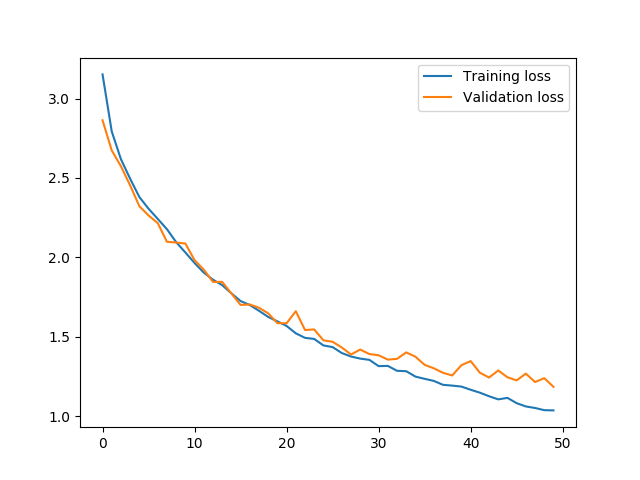
\includegraphics[scale=0.4]{img/batch-pre-loss.png}
    \subcaption{Evolución de la función de pérdida.}
    \label{fig:batch-pre-loss}
  \end{subfigure}%
  ~ \quad
  \begin{subfigure}{.5\textwidth}
    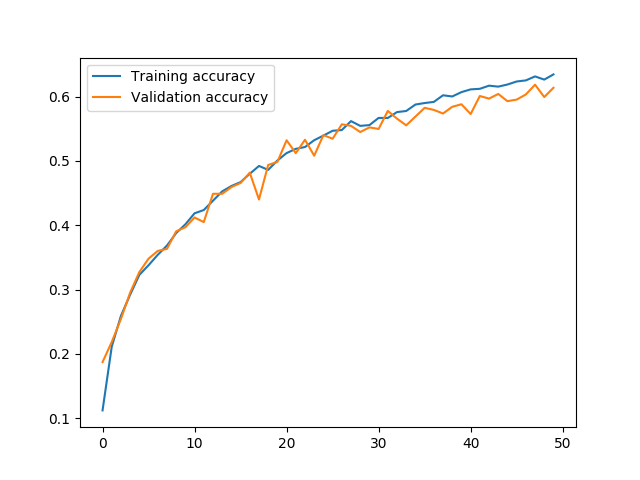
\includegraphics[scale=0.4]{img/batch-pre-acc.png}
    \subcaption{Evolución de la \textit{accuracy}.}
    \label{fig:batch-pre-acc}
  \end{subfigure}
  \caption{Historia del \textit{Modelo Pre}.}
  \label{fig:history-batch-pre}
\end{figure}

\begin{figure}[H]
  \centering
  \begin{subfigure}{.5\textwidth}
    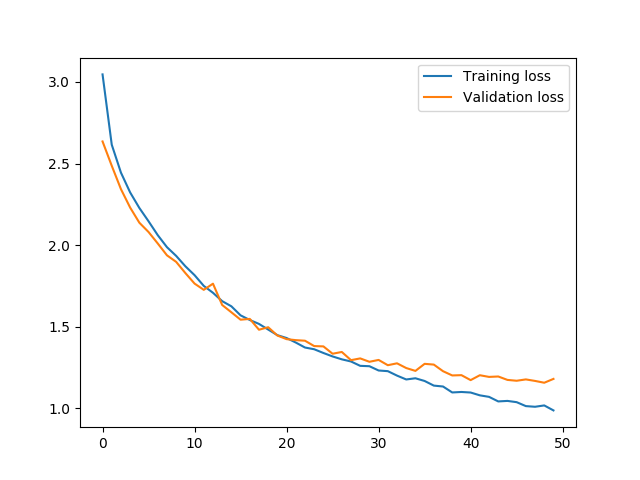
\includegraphics[scale=0.4]{img/batch-post-loss.png}
    \subcaption{Evolución de la función de pérdida.}
    \label{fig:batch-post-loss}
  \end{subfigure}%
  ~ \quad
  \begin{subfigure}{.5\textwidth}
    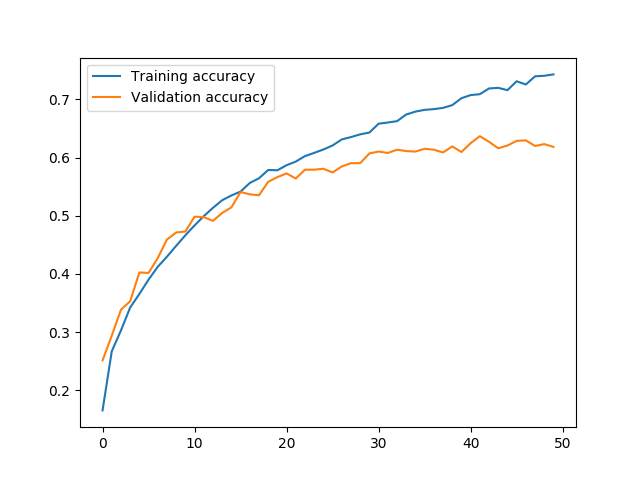
\includegraphics[scale=0.4]{img/batch-post-acc.png}
    \subcaption{Evolución de la \textit{accuracy}.}
    \label{fig:batch-post-acc}
  \end{subfigure}
  \caption{Historia del \textit{Modelo Post}.}
  \label{fig:history-batch-post}
\end{figure}

Observando las gráficas, podemos ver claramente que los resultados que han obtenido ambos
modelos en el conjunto de validación son muy buenos, ya que son casi idénticos a los obtenidos
en el conjunto de entrenamiento. Podemos ver que en ambos casos existe muy poca discrepancia,
ya que, a medida que los resultados mejoran en el conjunto de entrenamiento, sucede lo mismo
en el conjunto de validación. Sin embargo, es importante destacar que en las últimas épocas
del \textit{Modelo Post} los resultados de validación empiezan a separarse un poco de los
obtenidos en entrenamiento. En cambio, esto no sucede en el \textit{Modelo Pre}, ya que los
resultados en validación se ajustan más a los obtenidos en entrenamiento.

En general, los resultados obtenidos por estos modelos son los mejores que se han obtenido
hasta ahora. En ambos casos los valores de la función de pérdida se sitúan por debajo de 1.5,
y la precisión ronda aproximadamente 0.6.

Elegir el mejor modelo entre los dos puede ser difícil ya que ambos ofrecen unos excelentes
resultados. No obstante, vamos a quedarnos con el \textbf{\textit{Modelo Pre}}, ya que los resultados
parecen ser un poco más consistentes que los obtenidos en el \textit{Modelo Post}. Además de eso,
creemos que tiene más sentido realizar la normalización antes de la función de activación RELU.

Por ejemplo, si todos los valores de salida de una capa fuesen negativos y éstos tuviesen que pasar
por una función de activación como por ejemplo RELU, todos ellos serían puestos a 0, ya que en esta
función lo que se hace normalmente es conservar los valores positivos y poner los negativos a 0.
De esta forma, todas las conexiones estarían desactivadas, y no se podría hacer nada más. Al normalizar
antes, los valores pasarán a tener media $\mu = 0$ y desviación típica $\sigma = 1$, de tal forma
que habrán valores que permanezcan activos después de la función de activación, ya que tendremos
valores positivos.


\subsection{Ajuste del modelo final}

Habiendo escogido el \textit{Modelo Pre} como mejor modelo, ya solo nos queda ver de qué es capaz
con el conjunto de test. También, si nos fijamos en los resultados que se pueden ver en
\ref{fig:history-batch-pre}, podemos ver que todavía hay cierto margen de mejora. Por tanto,
vamos a realizar el ajuste final del modelo en un número superior de épocas. Vamos a fijar
este valor a 60, ya que creemos que es un número lo suficientemente grande como para permitir
sacarle todo el potencial a nuestro modelo.

Antes de entrenar de nuevo el modelo, vamos a hacer una serie de cosas. Lo primero, vamos
a crear un generador de datos para el conjunto de test. Este generador solo tiene que hacer
la normalización, ya que en el conjunto de test \textbf{nunca} debemos hacer aumento de datos.
Por tanto, declaramos nuestro generador de la siguiente forma:

\begin{lstlisting}
# Crear generador de test
datagen_test = ImageDataGenerator(
    featurewise_center=True,
    featurewise_std_normalization=True
)
\end{lstlisting}

Habiendo declarado el generador, hace falta entrenarlo. Para ello, tenemos que utilizar los
datos del conjunto de entrenamiento, ya que la normalización a los datos de test debe hacerse
en función de los datos con los que se ha entrenado, porque los datos de test son desconocidos
para nuestro modelo. El entrenamiento del generador se lleva a cabo de la siguiente manera:

\begin{lstlisting}
# Entrenar generador
datagen_test.fit(x_train)
\end{lstlisting}

Y, finalemnte, antes de proceder con el ajuste final, vamos a ver cómo queda la arquitectura del
modelo final:

\begin{figure}[H]
  \centering
  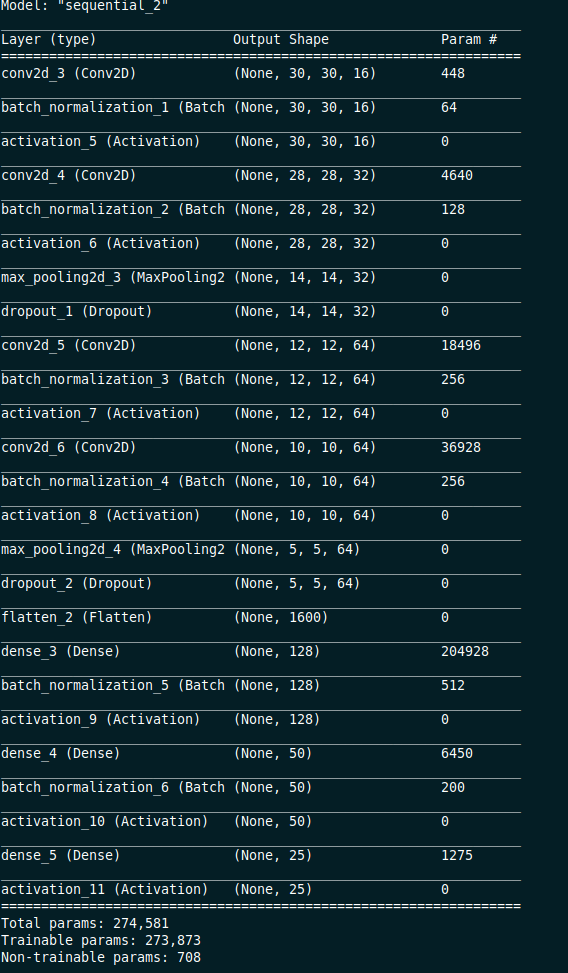
\includegraphics[scale=0.4]{img/final-model.png}
  \caption{Arquitectura del modelo final.}
  \label{fig:final-model}
\end{figure}

Como se puede ver, es una red con bastantes parámetros para la profundiad que tiene. Aunque en
un principio se ven muchas capas, solo unas pocas de ellas son las que realmente hacen operaciones
sobre imágenes (solo hay 4). El resto añaden regularización al modelo o son las capas densas.

Una vez visto esto, vamos a proceder al entrenamiento final. Para hacerlo, utilizamos el generador
de \textit{flip} que habíamos definido anteriormente:

\begin{lstlisting}
# Entrenar modelo utilizando aumento de datos
history = model_batch_pre.fit_generator(
    train_iter_flip,
    steps_per_epoch=len(x_train)*0.9/batch_size,
    epochs=epochs,
    validation_data=validation_iter_flip,
    validation_steps=len(x_train)*0.1/batch_size
)
\end{lstlisting}

De nuevo, podemos ver la historia de este modelo, la cuál viene dada por las siguientes gráficas:

\begin{figure}[H]
  \centering
  \begin{subfigure}{.5\textwidth}
    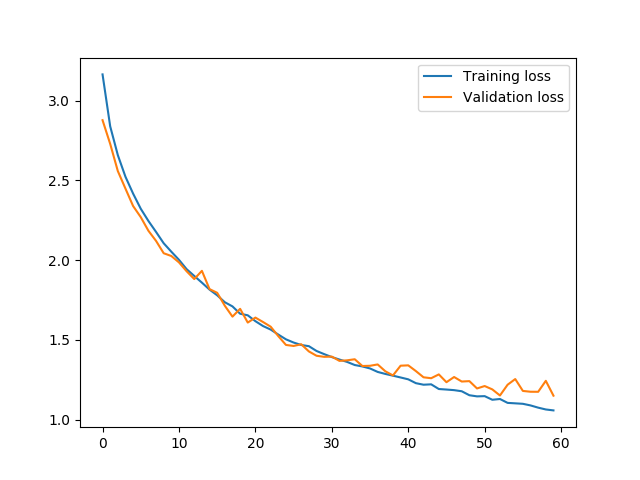
\includegraphics[scale=0.4]{img/final-loss.png}
    \subcaption{Evolución de la función de pérdida.}
    \label{fig:final-loss}
  \end{subfigure}%
  ~ \quad
  \begin{subfigure}{.5\textwidth}
    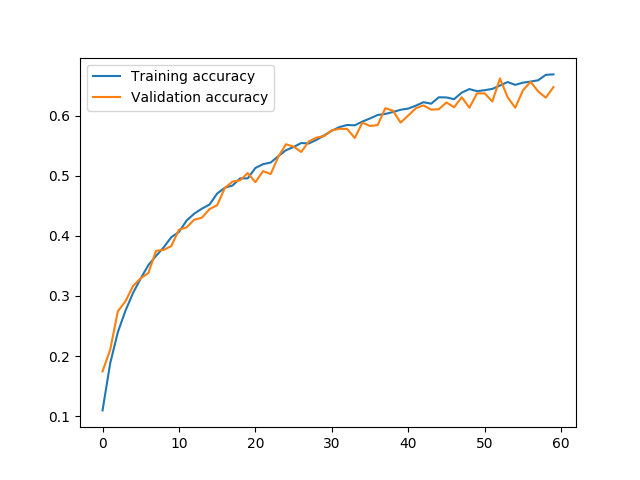
\includegraphics[scale=0.4]{img/final-acc.png}
    \subcaption{Evolución de la \textit{accuracy}.}
    \label{fig:final-acc}
  \end{subfigure}
  \caption{Historia del \textit{Modelo Pre}.}
  \label{fig:history-final}
\end{figure}

Podemos ver como el ajuste es muy bueno, ya que los valores obtenidos en el conjunto de validación
son casi idénticos a los obtenidos en el conjunto de entrenamiento. No hay mucha diferencia notable
entre los resultados obtenidos en ambos conjuntos. Además, el valor de la función de pérdida obtenido es el más
bajo hasta el momento, acercándose a 1 en las últimas épocas, y la precisión está por encima de 0.6.
Aparte, vemos claramente que el modelo no padece ni de \textit{underfit} ni de \textit{overfit}, ya que
ha sido regularizado previamente.

A la vista de los resultados obtenidos, podemos decir que el modelo tiene una muy buena capacidad
de generalización, y que muy posiblemente los resultados obtenidos en el conjunto de test sean
muy próximos a los obtenidos en el conjunto de validación.

Para predecir las etiquetas, podemos utilizar el método $predict\_generator()$ de la clase
$ImageDataGenerator$. La llamada al método sería la siguiente:

\begin{lstlisting}
# Predecir los datos
prediction = model_batch_pre.predict_generator(
    datagen_test.flow(x_test, batch_size=1, shuffle=False),
    steps=len(x_test),
    verbose=1
)
\end{lstlisting}

Este método recibe un iterador del generador, al cuál se le pasa el conjunto de datos $x\_test$, un 
tamaño de \textit{batch} (en este caso es 1, ya que los elementos se van a predecir de uno en uno) y
el parámetro $shuffle$ a \textbf{False}, de forma que no se barajen los datos y salgan en el mismo orden
(esto es importante para luego poder comparar con las etiquetas reales, ya que sino se desordenarían
los datos de salida y no habría forma de comparar las etiquetas predichas a las reales). Adicionalmente,
se dice que se den tantos pasos como elementos en el conjunto de test haya, y con $verbose = 1$ se solicita
que se muestre el progreso.

Una vez hemos predicho las etiquetas, podemos calcular la precisión de nuestro modelo comparando los valores
predichos con los reales. Para ello, nos podemos servir de la función que se nos ha proporcionado. Por tanto,
se resumiría en hacer la siguiente llamada:

\begin{lstlisting}
# Obtener accuracy de test
accuracy = calcularAccuracy(y_test, prediction)
\end{lstlisting}

En este caso se ha obtenido una \textit{accuracy} de 0.664, un valor bastante elevado teniendo en cuenta
de que partíamos de aproximadamente 0.4. Por tanto, ha habido una mejora de aproximadmente el 60\% en
la precisión. Esto nos indica que todas las mejoras que hemos hecho han tenido su efecto, y que por tanto,
hemos tomado la decisión correcta al incorporarlas al modelo.

\section{\textsc{Transferencia de modelos y ajuste fino con ResNet50 para la base de datos Caltech-UCSD}}

\subsection{ResNet50 como extractor de características}

Podemos utilizar la red ResNet50 como extractor de características aprovechando que ya ha sido
entrenada y, con las características que se obtengan, entrenar un modelo simple de clasificación.

Podemos declarar el modelo ResNet50 preentrenado que utilizaremos para extraer las características
de las imágenes de la siguiente manera:

\begin{lstlisting}
# Definir el modelo ResNet50 (preentrenado en ImageNet y sin la ultima capa).
resnet50 = ResNet50(include_top=False, weights='imagenet',
					pooling='avg')
\end{lstlisting}

De esta forma, al poner el parámetro $include\_top$ a \textbf{False} se le quita al modelo
que proporciona Keras la última capa, la cuál es una capa totalmente conectada que no nos
interesa tener, ya que utilizaremos nuestro propio clasificador. El parámetro $weights = imagenet$
indica que queremos cargar la red ya preentrenada en el conjunto de datos ImageNet.
El último parámetro, $pooling = avg$ indica que se va a coger la salida del último bloque
convolucional y se le va a aplicar una media global. Es decir, se va a calcular
la media de cada imagen, y eso será un elemento del vector de salida. Dicho vector
tendrá un tamaño de 2048 posiciones, y será el vector de características que sirva de
entrada a nuestro clasificador.

\subsection{Ajuste fino de ResNet50}

\newpage

\bibliographystyle{plain}
\bibliography{mybib}

\end{document}

